
%% bare_conf.tex
%% V1.3
%% 2007/01/11
%% by Michael Shell
%% See:
%% http://www.michaelshell.org/
%% for current contact information.
%%
%% This is a skeleton file demonstrating the use of IEEEtran.cls
%% (requires IEEEtran.cls version 1.7 or later) with an IEEE conference paper.
%%
%% Support sites:
%% http://www.michaelshell.org/tex/ieeetran/
%% http://www.ctan.org/tex-archive/macros/latex/contrib/IEEEtran/
%% and
%% http://www.ieee.org/

%%*************************************************************************
%% Legal Notice:
%% This code is offered as-is without any warranty either expressed or
%% implied; without even the implied warranty of MERCHANTABILITY or
%% FITNESS FOR A PARTICULAR PURPOSE! 
%% User assumes all risk.
%% In no event shall IEEE or any contributor to this code be liable for
%% any damages or losses, including, but not limited to, incidental,
%% consequential, or any other damages, resulting from the use or misuse
%% of any information contained here.
%%
%% All comments are the opinions of their respective authors and are not
%% necessarily endorsed by the IEEE.
%%
%% This work is distributed under the LaTeX Project Public License (LPPL)
%% ( http://www.latex-project.org/ ) version 1.3, and may be freely used,
%% distributed and modified. A copy of the LPPL, version 1.3, is included
%% in the base LaTeX documentation of all distributions of LaTeX released
%% 2003/12/01 or later.
%% Retain all contribution notices and credits.
%% ** Modified files should be clearly indicated as such, including  **
%% ** renaming them and changing author support contact information. **
%%
%% File list of work: IEEEtran.cls, IEEEtran_HOWTO.pdf, bare_adv.tex,
%%                    bare_conf.tex, bare_jrnl.tex, bare_jrnl_compsoc.tex
%%*************************************************************************

% *** Authors should verify (and, if needed, correct) their LaTeX system  ***
% *** with the testflow diagnostic prior to trusting their LaTeX platform ***
% *** with production work. IEEE's font choices can trigger bugs that do  ***
% *** not appear when using other class files.                            ***
% The testflow support page is at:
% http://www.michaelshell.org/tex/testflow/



% Note that the a4paper option is mainly intended so that authors in
% countries using A4 can easily print to A4 and see how their papers will
% look in print - the typesetting of the document will not typically be
% affected with changes in paper size (but the bottom and side margins will).
% Use the testflow package mentioned above to verify correct handling of
% both paper sizes by the user's LaTeX system.
%
% Also note that the "draftcls" or "draftclsnofoot", not "draft", option
% should be used if it is desired that the figures are to be displayed in
% draft mode.
%
\documentclass[conference]{IEEEtran}
% Add the compsoc option for Computer Society conferences.
%
% If IEEEtran.cls has not been installed into the LaTeX system files,
% manually specify the path to it like:
% \documentclass[conference]{../sty/IEEEtran}





% Some very useful LaTeX packages include:
% (uncomment the ones you want to load)


% *** MISC UTILITY PACKAGES ***
%
%\usepackage{ifpdf}
% Heiko Oberdiek's ifpdf.sty is very useful if you need conditional
% compilation based on whether the output is pdf or dvi.
% usage:
% \ifpdf
%   % pdf code
% \else
%   % dvi code
% \fi
% The latest version of ifpdf.sty can be obtained from:
% http://www.ctan.org/tex-archive/macros/latex/contrib/oberdiek/
% Also, note that IEEEtran.cls V1.7 and later provides a builtin
% \ifCLASSINFOpdf conditional that works the same way.
% When switching from latex to pdflatex and vice-versa, the compiler may
% have to be run twice to clear warning/error messages.






% *** CITATION PACKAGES ***
%
%\usepackage{cite}
% cite.sty was written by Donald Arseneau
% V1.6 and later of IEEEtran pre-defines the format of the cite.sty package
% \cite{} output to follow that of IEEE. Loading the cite package will
% result in citation numbers being automatically sorted and properly
% "compressed/ranged". e.g., [1], [9], [2], [7], [5], [6] without using
% cite.sty will become [1], [2], [5]--[7], [9] using cite.sty. cite.sty's
% \cite will automatically add leading space, if needed. Use cite.sty's
% noadjust option (cite.sty V3.8 and later) if you want to turn this off.
% cite.sty is already installed on most LaTeX systems. Be sure and use
% version 4.0 (2003-05-27) and later if using hyperref.sty. cite.sty does
% not currently provide for hyperlinked citations.
% The latest version can be obtained at:
% http://www.ctan.org/tex-archive/macros/latex/contrib/cite/
% The documentation is contained in the cite.sty file itself.






% *** GRAPHICS RELATED PACKAGES ***
%

\ifCLASSINFOpdf
   \usepackage[pdftex]{graphicx}
  % declare the path(s) where your graphic files are
   \graphicspath{{../pdf/}{../jpeg/}{../png/}}
  % and their extensions so you won't have to specify these with
  % every instance of \includegraphics
  \DeclareGraphicsExtensions{.pdf,.jpeg,.png}
  \usepackage[justification=centering]{caption}
\else
  % or other class option (dvipsone, dvipdf, if not using dvips). graphicx
  % will default to the driver specified in the system graphics.cfg if no
  % driver is specified.
  \usepackage[dvips]{graphicx}
  % declare the path(s) where your graphic files are
  \graphicspath{{../eps/}}
  % and their extensions so you won't have to specify these with
  % every instance of \includegraphics
  \DeclareGraphicsExtensions{.eps}
\fi
% graphicx was written by David Carlisle and Sebastian Rahtz. It is
% required if you want graphics, photos, etc. graphicx.sty is already
% installed on most LaTeX systems. The latest version and documentation can
% be obtained at: 
% http://www.ctan.org/tex-archive/macros/latex/required/graphics/
% Another good source of documentation is "Using Imported Graphics in
% LaTeX2e" by Keith Reckdahl which can be found as epslatex.ps or
% epslatex.pdf at: http://www.ctan.org/tex-archive/info/
%
% latex, and pdflatex in dvi mode, support graphics in encapsulated
% postscript (.eps) format. pdflatex in pdf mode supports graphics
% in .pdf, .jpeg, .png and .mps (metapost) formats. Users should ensure
% that all non-photo figures use a vector format (.eps, .pdf, .mps) and
% not a bitmapped formats (.jpeg, .png). IEEE frowns on bitmapped formats
% which can result in "jaggedy"/blurry rendering of lines and letters as
% well as large increases in file sizes.
%
% You can find documentation about the pdfTeX application at:
% http://www.tug.org/applications/pdftex





% *** MATH PACKAGES ***
%
\usepackage[cmex10]{amsmath}
% A popular package from the American Mathematical Society that provides
% many useful and powerful commands for dealing with mathematics. If using
% it, be sure to load this package with the cmex10 option to ensure that
% only type 1 fonts will utilized at all point sizes. Without this option,
% it is possible that some math symbols, particularly those within
% footnotes, will be rendered in bitmap form which will result in a
% document that can not be IEEE Xplore compliant!
%
% Also, note that the amsmath package sets \interdisplaylinepenalty to 10000
% thus preventing page breaks from occurring within multiline equations. Use:
%\interdisplaylinepenalty=2500
% after loading amsmath to restore such page breaks as IEEEtran.cls normally
% does. amsmath.sty is already installed on most LaTeX systems. The latest
% version and documentation can be obtained at:
% http://www.ctan.org/tex-archive/macros/latex/required/amslatex/math/





% *** SPECIALIZED LIST PACKAGES ***
%
\usepackage{algorithm}
\usepackage{algorithmic}
% algorithmic.sty was written by Peter Williams and Rogerio Brito.
% This package provides an algorithmic environment fo describing algorithms.
% You can use the algorithmic environment in-text or within a figure
% environment to provide for a floating algorithm. Do NOT use the algorithm
% floating environment provided by algorithm.sty (by the same authors) or
% algorithm2e.sty (by Christophe Fiorio) as IEEE does not use dedicated
% algorithm float types and packages that provide these will not provide
% correct IEEE style captions. The latest version and documentation of
% algorithmic.sty can be obtained at:
% http://www.ctan.org/tex-archive/macros/latex/contrib/algorithms/
% There is also a support site at:
% http://algorithms.berlios.de/index.html
% Also of interest may be the (relatively newer and more customizable)
% algorithmicx.sty package by Szasz Janos:
% http://www.ctan.org/tex-archive/macros/latex/contrib/algorithmicx/




% *** ALIGNMENT PACKAGES ***
%
%\usepackage{array}
% Frank Mittelbach's and David Carlisle's array.sty patches and improves
% the standard LaTeX2e array and tabular environments to provide better
% appearance and additional user controls. As the default LaTeX2e table
% generation code is lacking to the point of almost being broken with
% respect to the quality of the end results, all users are strongly
% advised to use an enhanced (at the very least that provided by array.sty)
% set of table tools. array.sty is already installed on most systems. The
% latest version and documentation can be obtained at:
% http://www.ctan.org/tex-archive/macros/latex/required/tools/


%\usepackage{mdwmath}
%\usepackage{mdwtab}
% Also highly recommended is Mark Wooding's extremely powerful MDW tools,
% especially mdwmath.sty and mdwtab.sty which are used to format equations
% and tables, respectively. The MDWtools set is already installed on most
% LaTeX systems. The lastest version and documentation is available at:
% http://www.ctan.org/tex-archive/macros/latex/contrib/mdwtools/


% IEEEtran contains the IEEEeqnarray family of commands that can be used to
% generate multiline equations as well as matrices, tables, etc., of high
% quality.


%\usepackage{eqparbox}
% Also of notable interest is Scott Pakin's eqparbox package for creating
% (automatically sized) equal width boxes - aka "natural width parboxes".
% Available at:
% http://www.ctan.org/tex-archive/macros/latex/contrib/eqparbox/





% *** SUBFIGURE PACKAGES ***
%\usepackage[tight,footnotesize]{subfigure}
% subfigure.sty was written by Steven Douglas Cochran. This package makes it
% easy to put subfigures in your figures. e.g., "Figure 1a and 1b". For IEEE
% work, it is a good idea to load it with the tight package option to reduce
% the amount of white space around the subfigures. subfigure.sty is already
% installed on most LaTeX systems. The latest version and documentation can
% be obtained at:
% http://www.ctan.org/tex-archive/obsolete/macros/latex/contrib/subfigure/
% subfigure.sty has been superceeded by subfig.sty.



%\usepackage[caption=false]{caption}
%\usepackage[font=footnotesize]{subfig}
% subfig.sty, also written by Steven Douglas Cochran, is the modern
% replacement for subfigure.sty. However, subfig.sty requires and
% automatically loads Axel Sommerfeldt's caption.sty which will override
% IEEEtran.cls handling of captions and this will result in nonIEEE style
% figure/table captions. To prevent this problem, be sure and preload
% caption.sty with its "caption=false" package option. This is will preserve
% IEEEtran.cls handing of captions. Version 1.3 (2005/06/28) and later 
% (recommended due to many improvements over 1.2) of subfig.sty supports
% the caption=false option directly:
%\usepackage[caption=false,font=footnotesize]{subfig}
%
% The latest version and documentation can be obtained at:
% http://www.ctan.org/tex-archive/macros/latex/contrib/subfig/
% The latest version and documentation of caption.sty can be obtained at:
% http://www.ctan.org/tex-archive/macros/latex/contrib/caption/




% *** FLOAT PACKAGES ***
%
%\usepackage{fixltx2e}
% fixltx2e, the successor to the earlier fix2col.sty, was written by
% Frank Mittelbach and David Carlisle. This package corrects a few problems
% in the LaTeX2e kernel, the most notable of which is that in current
% LaTeX2e releases, the ordering of single and double column floats is not
% guaranteed to be preserved. Thus, an unpatched LaTeX2e can allow a
% single column figure to be placed prior to an earlier double column
% figure. The latest version and documentation can be found at:
% http://www.ctan.org/tex-archive/macros/latex/base/



%\usepackage{stfloats}
% stfloats.sty was written by Sigitas Tolusis. This package gives LaTeX2e
% the ability to do double column floats at the bottom of the page as well
% as the top. (e.g., "\begin{figure*}[!b]" is not normally possible in
% LaTeX2e). It also provides a command:
%\fnbelowfloat
% to enable the placement of footnotes below bottom floats (the standard
% LaTeX2e kernel puts them above bottom floats). This is an invasive package
% which rewrites many portions of the LaTeX2e float routines. It may not work
% with other packages that modify the LaTeX2e float routines. The latest
% version and documentation can be obtained at:
% http://www.ctan.org/tex-archive/macros/latex/contrib/sttools/
% Documentation is contained in the stfloats.sty comments as well as in the
% presfull.pdf file. Do not use the stfloats baselinefloat ability as IEEE
% does not allow \baselineskip to stretch. Authors submitting work to the
% IEEE should note that IEEE rarely uses double column equations and
% that authors should try to avoid such use. Do not be tempted to use the
% cuted.sty or midfloat.sty packages (also by Sigitas Tolusis) as IEEE does
% not format its papers in such ways.





% *** PDF, URL AND HYPERLINK PACKAGES ***
%
%\usepackage{url}
% url.sty was written by Donald Arseneau. It provides better support for
% handling and breaking URLs. url.sty is already installed on most LaTeX
% systems. The latest version can be obtained at:
% http://www.ctan.org/tex-archive/macros/latex/contrib/misc/
% Read the url.sty source comments for usage information. Basically,
% \url{my_url_here}.





% *** Do not adjust lengths that control margins, column widths, etc. ***
% *** Do not use packages that alter fonts (such as pslatex).         ***
% There should be no need to do such things with IEEEtran.cls V1.6 and later.
% (Unless specifically asked to do so by the journal or conference you plan
% to submit to, of course. )


% correct bad hyphenation here
\hyphenation{op-tical net-works semi-conduc-tor}


\begin{document}
%
% paper title
% can use linebreaks \\ within to get better formatting as desired
\title{Taking One Small Step Forward:\\Finding Low-Frequentcy Items in Data Streams}


% author names and affiliations
% use a multiple column layout for up to three different
% affiliations
\author{\IEEEauthorblockN{Michael Shell}
\IEEEauthorblockA{School of Electrical and\\Computer Engineering\\
Georgia Institute of Technology\\
Atlanta, Georgia 30332--0250\\
Email: http://www.michaelshell.org/contact.html}
\and
\IEEEauthorblockN{Homer Simpson}
\IEEEauthorblockA{Twentieth Century Fox\\
Springfield, USA\\
Email: homer@thesimpsons.com}
\and
\IEEEauthorblockN{James Kirk\\ and Montgomery Scott}
\IEEEauthorblockA{Starfleet Academy\\
San Francisco, California 96678-2391\\
Telephone: (800) 555--1212\\
Fax: (888) 555--1212}}

% conference papers do not typically use \thanks and this command
% is locked out in conference mode. If really needed, such as for
% the acknowledgment of grants, issue a \IEEEoverridecommandlockouts
% after \documentclass

% for over three affiliations, or if they all won't fit within the width
% of the page, use this alternative format:
% 
%\author{\IEEEauthorblockN{Michael Shell\IEEEauthorrefmark{1},
%Homer Simpson\IEEEauthorrefmark{2},
%James Kirk\IEEEauthorrefmark{3}, 
%Montgomery Scott\IEEEauthorrefmark{3} and
%Eldon Tyrell\IEEEauthorrefmark{4}}
%\IEEEauthorblockA{\IEEEauthorrefmark{1}School of Electrical and Computer Engineering\\
%Georgia Institute of Technology,
%Atlanta, Georgia 30332--0250\\ Email: see http://www.michaelshell.org/contact.html}
%\IEEEauthorblockA{\IEEEauthorrefmark{2}Twentieth Century Fox, Springfield, USA\\
%Email: homer@thesimpsons.com}
%\IEEEauthorblockA{\IEEEauthorrefmark{3}Starfleet Academy, San Francisco, California 96678-2391\\
%Telephone: (800) 555--1212, Fax: (888) 555--1212}
%\IEEEauthorblockA{\IEEEauthorrefmark{4}Tyrell Inc., 123 Replicant Street, Los Angeles, California 90210--4321}}




% use for special paper notices
%\IEEEspecialpapernotice{(Invited Paper)}




% make the title area
\maketitle


\begin{abstract}
%\boldmath
Low-frequency items in data streams are becoming more and more important due to their large amount, and the ability to excavate the rich information contained in them is of great significance to many companies and organizations. We propose an one-pass algorithm, called \emph{BFSS}, which can identify items in a data stream with frequencies less than a user specified support. Our algorithm is simple and have provably small memory footprints related to domain of data streams. Although the output is approximate, we can guarantee no false negatives and provably few false positives. Given a little modification, \emph{BFSS} can be improved to \emph{SBFSS}, which can handle low-frequency items detection over data streams from large domain with acceptable and bounded false negatives and false positives using a proper space.
\end{abstract}
% IEEEtran.cls defaults to using nonbold math in the Abstract.
% This preserves the distinction between vectors and scalars. However,
% if the conference you are submitting to favors bold math in the abstract,
% then you can use LaTeX's standard command \boldmath at the very start
% of the abstract to achieve this. Many IEEE journals/conferences frown on
% math in the abstract anyway.

% no keywords




% For peer review papers, you can put extra information on the cover
% page as needed:
% \ifCLASSOPTIONpeerreview
% \begin{center} \bfseries EDICS Category: 3-BBND \end{center}
% \fi
%
% For peerreview papers, this IEEEtran command inserts a page break and
% creates the second title. It will be ignored for other modes.
\IEEEpeerreviewmaketitle



\section{Introduction}
% no \IEEEPARstart
In many real-world applications, information such as web click data, stock ticker
data, sensor network data, phone call records, and traffic monitoring data appear in the form
of data streams. Online monitoring of data streams has emerged as an important research
undertaking. Estimating the frequency of the items on these streams is an important aggregation and summary technique for both stream mining and data management systems with a broad range of applications. A variety of algorithms have been proposed to identify frequent items from data streams, \emph{Sticky Sampling} [] and \emph{Space Saving} [] etc.\par
However, to the best of our knowledge, there are no algorithms identifying low-frequency items over data streams. Low-frequency items, similar to the defination of frequent items, are items frequencies of which are less than a specified threshold S. \par
Zipf's law refers to the fact that many types of data studied in the physical and social sciences can be approximated with a Zipfian distribution, one of a family of related discrete power law distributions. Fig.\ref{fig:sim} describes relation between frequency rank and frequency of items that follow a power law distribution over data streams, and we can find that the distinct number of low-frequency items is much larger than the distinct number of frequent items, so under the restriction of limited memory it is much more difficult to identify low-frequency items than to identify frequent items. \par
Nowadays, Low-frequency items over data streams are becoming more and more important because of the rich information they contain which can be easily understood through the observation of entropy of data streams []. We take one small step forward to maintain low-frequency items over data streams approximately and try to fill up the blank of low-frequency items mining over data streams in this paper.   
% You must have at least 2 lines in the paragreaph with the drop letter
% (should never be an issue)

\begin{figure}
	\centering
	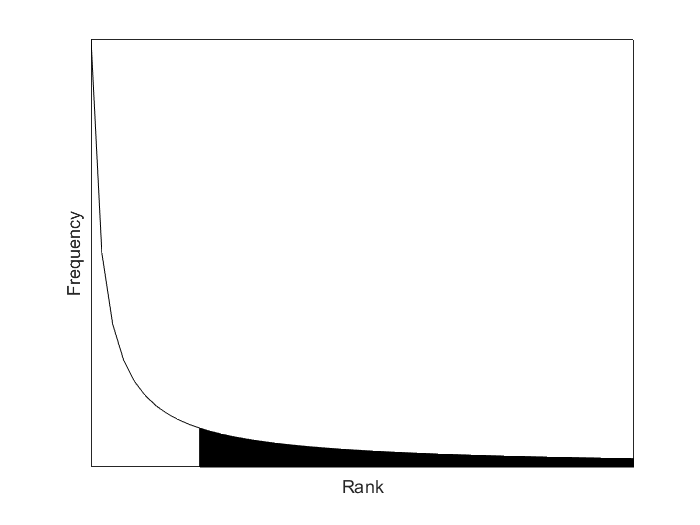
\includegraphics[width=2.5in]{png/zipf.png}
	\caption{Rank-frequency distribution}
	\label{fig:sim}
\end{figure}


\subsection{Motivating Examples}
\subsubsection{Individual requirements mining}
In such an era that information technology develops rapidly, it is much easier for us to get access to various of knowledge and information and we need through a few mouse clicks, for example, we can shop online with the help of e-commerce site, such as Amazon and Taobao etc. We can search whatever we are interested in through search engines, such as Google and Bing etc. \par 
Our requirements are popular most times, for example, buying a regular water glass online or searching the information about a tourist attraction etc, and these popular requirements can be easily met because almost every e-commerce site sell all linds of water glasses and nearly every search engines provide links to popular tourist attractions worldwide.  \par
However, we are no longer saiesfied with responses only to popular demands. For example, it is not so easy for us to buy embroidery stitches online or search information about a nameless small village in China, because these are individual requirements, and some e-commerce sites or search engines may neglect these requirements, for example, i can't find product information about embroidery stitches at Amazon while Taobao does. \par
Yusuf Mehdi, SVP of Microsoft, once said at the meeting of Search Engine Strategies in 2010 that major reason why Bing got begind with Google is neglecting ``long tail'' of search flow items of which appear a few times or even once, and it is of great importance for them to analyze these low-frequency items. So it is individual requirements or in other words low-frequency demands, in some sense, that really make a difference rather than popular demands in areas like e-commerce and SE, and identifying them is the first step to do deep analysis on them.

\subsubsection{Data distribution estimation}
Data distribution is a basic and important property of a data stream. Sampling is a simple and fast method to estimate data distributions, however, sampling will lose much inforamtion of data streams and cause big errors sometimes. From Figure \ref{fig:sim}, we can observe that low-frequency elements have a great influence on data distributions of most data streams, in fact, low-frequency elements dominate the distinct elements in data streams of various distributions which can be seen in our experiments. \par 
In fact, \emph{BFSS} and \emph{SBFSS} can find both frequent and low-frequency items in data streams efficiently, and in this way we can get much more accurate estimates of data distributions of data streams.

\subsection{Our Contributions}
We introduce and state the proplem of low-frequency items detection over data streams which are of great significance in areas such as individual requirements mining and data distribution estimation, and to the best of our knowledge there is no relative research up to now.\par

In this paper, we propose \emph{BFSS}, which extends the classic frequent items detection algorithm \emph{Space Saving} to maintain both frequent and low-frequency items in a data stream approximately. The basic idea of our solution is as follows: each item in a data stream is either a frequent one or a low-frequency one once the threshold $\phi[\in (0,1)]$ is set, so we can maintain low-frequency items by filtering the frequent items out. A major problem we have to deal with is to maintain an itemset items in which appear in the data stream, and this can be done approximately using a Bloom filter size of which is related to the size of domain of data streams. \emph{BFSS} gurantee no false negatives and provably few false positives using small memory footprints.\par

However, size of a Bloom filter must increase with the size of domain in order to keep a low false positive rate, and here comes a problem: what if the domain is too large to be handled by a Bloom filter in a limited space? Inspired by the solution presented in [], we propose \emph{SBFSS} which extends \emph{BFSS} to deal with data streams from large domains, and \emph{SBFSS} gurantee acceptable and bounded false negatives and false positives using a proper space.

\subsection{Roadmap}
In Section 2, we present the problem statement and some background on existing approches which deal with the problem of frequent items detection. Our solutions are presented and discussed in Section 3. In Section 4, we experimentally evaluate out methods. Conclusions are given in Section 5.

\section{PRELIMINARIES}
This section presents the problem statement and some representative algorithms solvimg $\epsilon$\emph{-Deficient Frequent Elements} [sticky sampling] which will be formally defined below.Table \ref{tab:list} summarizes the major notation in this paper.

\begin{table}
	
    \caption{Major Notation Used in the Paper.}
   
	\begin{tabular}{ll}
		\hline	Notation  & Meaning\\ 
		\hline
		\emph{BFSS} & Our first algorithm\\
		\emph{SBFSS} & Our second algorithm\\	
		$S$ & The input data stream\\
		$A$ & The domain of $S$\\
		$M$ & The size of $A$\\
		$M'$ & The number of distinct elements in $S$\\
		$\phi$ & The user specified support threshold\\
		$D$ & The synopsis used in \emph{BFSS} and \emph{SBFSS}\\
	    $(e,f(e),\Delta(e))$ & The form of each counter in $D$\\ 
		$E$ & The set of elements monitored in $D$\\
		$min$ & The minimum value of $f(e)$ in $D$\\
		$C$ & The maximum number of counters in $D$\\
		$m$ & The number of counters used in $D$\\
		$N$ & The number of elements in the input stream\\
		$H$ & The number of hash functions used in \emph{BFSS} and \emph{SBFSS}\\
		$f_S(e)$ & The frequency of element $e$ in $S$\\ 
		\emph{FPs} &The elements in $S$ with frequency no less than $\lfloor \phi N\rfloor$\\& wrongly output\\
		\emph{FNs} & The elements in $S$ with frequency less than $\lfloor \phi N\rfloor$ \\&wrongly neglected\\
		\emph{BF}  &The Bloom filter used in \emph{BFSS}\\
		$K$ & The size of \emph{BF}\\
       \emph{SBF} &The Stable Bloom filter used in \emph{SBFSS}\\
        $K'$ & The size of \emph{SBF}\\
        $k$  &  Number of cells used in \emph{SBF}\\
        $d$  & Number of bits allocated per cell\\
        $max$ & The value a cell is set to\\
        $P$ &  Number of cells we pick to decrement by 1 in each iteration\\
        $p$ &  The probability that a cell is picked to be decremented by 1 \\
        &in each iteration\\
        $p'$ &  The probability that a cell is set in each iteration\\
       \hline
	\end{tabular}
\label{tab:list}

\end{table}

\subsection{Problem Statement}
Consider an input stream $S = e_1,e_2,..., e_N$ of current length $N$, which arrives item by item. Let each item $e_i$ belong to a universe set $A=\{a_1,a_2,...,a_M\}$ of size $M$ representing the input stream's domain. Let $f_S(a)$ denote the number of occurrences of $a$ in $S$\par

Our problem $\phi$\emph{-Bounded Low-Frequency Elements} can be stated as follows: given a data stream $S$ along with its domain $A$ and a user specified threshold $\phi[\in (0,1)]$, output the subset $I(S,\phi) \subset A$ of symbols defined as $I(S,\phi) = \{a\in A : 0 < f_S(a)\leq\lfloor \phi N\rfloor\}$.\par

At any point of time, \emph{BFSS} output a list of items with the following guarantees: 
\begin{enumerate}
\item  All elements whose true frequency is no more than $\lfloor\phi N\rfloor$ are output. There are \emph{no false negatives}.
\item  No element whose true frequency exceeds $2\lfloor\phi N\rfloor$ is output.
\end{enumerate} 

As for data streams from large domains which means $M$ is so large that \emph{BFSS} can not handle in mempry, \emph{SBFSS} output a list of items using proper space under the restriction of limited memory with acceptable false negatives and false positives, where a false positive is an item with frequency more than $\lfloor\phi N\rfloor$ wrongly output, and a false negative is an item with frequency no more than $\lfloor\phi N\rfloor$ wrongly neglected.

\subsection{Related Work}
As far as we know that there are no related algorithms addressing this problem, however, the methods we propose are based on algorithm solving $\epsilon$\emph{-Deficient Frequent Elements} which can be described as follows: given a input stream $S$ of current length $N$ and a support threshold $\phi \in (0,1)$, return the items whose frequencies are guaranteed to be no smaller than $\lfloor(\phi-\epsilon)N\rfloor$ deterministically or with a probability of at least $1-\delta$, where $\epsilon \in (0,1)$ is a user-defined error and $\delta \in (0,1)$ is a probability of failure, so we examine several algorithms solving $\epsilon$\emph{-Deficient Frequent Elements}.\par

research can be divided into two groups: \emph{counter-based} techniques and \emph{sketch-based} techniques.\par

\textbf{Counter-Based Techniques} keep an individual counter for each element in the monitored set, a subset of A. The counter of a monitored element, $e_i$, is updated when $e_i$ occurs in the stream. If there is no counter kept for the observed ID, it is either disregarded, or some algorithm-dependent action is taken.\par

Two representative algorithms \emph{Sticky Sampling} and \emph{Lossy Counting} were proposed in []. The algorithms cut the stream into rounds, and they prune some potential low-requency items at the edge of each round. Though simple and intuitive, they suffer from zeroing too many counters at rounds’ boundaries, and thus, they free space before it is really needed. In addition, answering a frequent elements query entails scanning all counters.\par

The algorithm \emph{Space-Saving} , the one we are based at, was proposed in []. The algorithm maintains a synopsis which keeps all counters in an order according to the value of each counter's monitoring frequency plus maximum possible error. For a non-monitored item, the counter with the smallest counts, \emph{min}, is assigned to monitor it, with the items monitoring frequency $f(e)$ set to 1 and its maximal possible error $\Delta(e)$ set to \emph{min}. Since $min\leq\epsilon N$ (this follows because of the choice of the number of counters), the operation amounts to replacing an old, potentially infrequent item with a new, hopefully frequent item. This strategy keeps the item information until the very end when space is absolutely needed, and it leads to the high accuracy of \emph{Space-Saving}. Experiments done in [overview] showed \emph{Space-Saving} outperforms other Counter-Based techniques in recall/precision tests.\par

\textbf{Sketch-Based Techniques} do not monitor a subset of elements, rather provide, with less stringent guarantees, frequency estimation for all elements using bitmaps of counters. Usually, each element is hashed into the space of counters using a family of hash functions, and the hashed-to counters are updated for every hit of this element. Those “representative” counters are then queried for the element frequency with less accuracy, due to hashing collisions.\par

The \emph{Count-Min Sketch} algorithm of Cormode and Muthukrishnan [Count-Min] maintains an array of $d\times w$ counters, and pairwise independent hash functions $h_j$ map items onto $[w]$ for each row. Each update is mapped onto $d$ entries in the array, each of which is incremented. The Markov inequality is used to show that the estimate for each $j$ overestimates by less than $n/w$, and repeating $d$ times reduces the probability of error exponentially.\par

The \emph{hCount} algorithm was proposed in []. The data structure and algorithms used in \emph{Count-Min Sketch} and \emph{hCount} shared the similarity, but were simultaneously and independently investigated with different focuses.

\section{OUR ALGORITHMS}
In this section, we will discuss our approaches \emph{BFSS} and \emph{SBFSS} in detail.
\subsection{The Challenges in $\phi$-Bounded Low-Frequency Elements}
$\phi$\emph{-Bounded Low-Frequency Elements} has two main challenges due to the different features between frequent items and low-frequency elements over data streams.\par

\textbf{The long tail phenomenon}. It can be easily proved that there are at most $\lceil1/\phi\rceil$ frequent elements whose frequency is more than $\lfloor\phi N\rfloor$ in any data stream, however, there is no provable upper bound of the number of low-frequency elements whose frequency is less than $\lfloor\phi N\rfloor$. In fact, our experiments on both real and synthetic data show that low-frequency elements occupy most of the distinct elements appear in data streams, and it is almost impossible to maintain all low-frequency elements in memory. Another observation is that their frequencies are very low and close as well, and it may consume much space to separate low-frequency elements from frequent elements especially when $\phi$ is very small.\par

\textbf{The unpredictability}. A basic and common idea of \emph{Counter-Based Techniques} is to discard potential infrequent elements dynamically, and it is based on the fact that potential infrequent elements will never become frequent elements if they don't appear afterwards, however, this fact no longer applies to low-frequency elements in data streams because potential elements will possibly become low-frequency elements if they don't appear afterwards. The unpredictability of low-frequency elements makes it difficult to maintain them directly like frequent elements.

\subsection{The BFSS Algorithm}\label{sec:bfss}
In consideration of the challenges in $\phi$\emph{-Bounded Low-Frequency Elements}, we tried to solve the problem indirectly by filtering frequent items out which is the underlying idea of \emph{BFSS}.\par
Two algorithms are proposed for updating and outputting final result separately. Algorithm \ref{alg:bfss} maintains a Bloom filter $BF$ of size $K$ with $H$ uniformly independent hash functions $\{h_1(x),...,h_H(x)\}$ and a synopsis $D$ with $M$ counters. Each of these $H$ hash function maps an element from $A$ to $[0,...,K-1]$. Initially each bit of BF is set to 0 and $D$ has $M$ empty counters. Each newly arrived element in the stream is mapped to $H$ bits in BF by the $H$ hash functions and we set the $H$ bits to 1. Then if we observe an element that is monitored in $D$, we just increment $f(e)$. If we observe an element, $e_{new}$, that is not monitored in $D$, handle it depending on whether there is an empty counter in $D$. If there is one, we just allocate it to $e_{new}$ and set $f(e_{new})$ to 1 and set $\Delta(e_{new})$ to 0. If $D$ is full, we just replace the element that currently has the least hits, $min$, with $e_{new}$. Assign $f(e_{new})$ the value $min+1$ and assign $\Delta(e_{new})$ the value $min$.\par

\begin{algorithm}[h]
	\caption{BFSS Update Algorithm}
	\label{alg:bfss}
\begin{algorithmic}[1]
	\REQUIRE Stream $S$, support threshold $\phi$
	\STATE $N=0,m=0,C=\lceil 1/\phi\rceil,K=\lambda',H=\mu'$; \COMMENT{$N$: length of stream; $m$: the number of counters used in $D$; $C$: the maximum number of counters in $D$; $K$: size of Bloom filter; $H$: number of hash functions;The value of $\lambda'$ and $\mu'$ will be discussed in detail later.}
	\STATE The form of the counters in $D$ is $(e,f(e),\Delta(e))$
	\FOR{$i=0$ to $K-1$}
	\STATE $BF[i]=0$
	\ENDFOR
	\FOR{each item $e$ of stream $S$}
	\FOR{$i=1$ to $H$}
	\STATE $BF[h_i(e)]=1$
	\ENDFOR
	\IF{$e$ is monitored in $D$}
	\STATE $f(e)=f(e)+1$;
	\ELSIF{$m<C$}
	\STATE Assign a new counter $(e,1,0)$ to it
	\STATE $m=m+1$
	\ELSE
	\STATE Let $e_m$ be the element with least hits, $min$
	\STATE Replace $e_m$ with $e$ in $D$
	\STATE $f(e)=min+1,\Delta(e)=min$
	\ENDIF
	\STATE $N=N+1$;
	\ENDFOR
\end{algorithmic}
\end{algorithm}

Algorithm \ref{alg:output} checks and outputs the element with frequency less than a user-specified threshold $\phi$. For each element in $A$, we first check whether it is in $BF$. If the element is not in $BF$, it must not be a low-frequency item because it never appeared in the stream. If the element is in $BF$ but not in $D$, it must be a low-frequency item and we output it, and we will give the reason later. If the element appears both in $BF$ and $D$, we identify the element as a low-frequency element if $f(e)<\lfloor \phi N\rfloor+\Delta(e)$ with high probability. The time requirement of Algorithm \ref{alg:output} is linear to the range of universe. It is acceptable when the frequency of the requests is not high. 

\begin{algorithm}[h]
	\caption{BFSS Query Algorithm}
	\label{alg:output}
	\begin{algorithmic}[1]
		\REQUIRE \emph{BF}, $D$, $\phi$, $A$, $N$, $M$
		\ENSURE low-frequency elements with threshold $\phi$
		\STATE $flag=true$; \COMMENT{ \emph{flag}: indicate whether an element is in \emph{BF} or not}
		\FOR{$i=0$ to $M-1$}
		\STATE $flag=true$
		\FOR{$j=1$ to $H$}
		\IF{$BF[h_j(A[i])]==0$}
		\STATE $flag=false$
		\STATE break;
		\ENDIF
		\ENDFOR
		\IF{$flag==true$}
		\IF{$A[i]$ is monitored in $D$}
		\IF{$f(A[i])\leq\lfloor \phi N\rfloor+\Delta(A[i])$}
		\STATE output $A[i]$ as a low-frequency element
		\ENDIF
		\ELSE
		\STATE output $A[i]$ as a low-frequency element
		\ENDIF
		\ENDIF
		\ENDFOR
	\end{algorithmic}
\end{algorithm}
\subsection{Analysis of BFSS}
In this section, we present a theoretical analysis of \emph{BFSS} described in Section \ref{sec:bfss}. We analyze \emph{FNs}, \emph{FPs}, space complexity, and time complexity. At last, we will identify the challenges to \emph{BFSS}. \par

\subsubsection{\textbf{Analysis of FNs}}
In this section, we will prove that there are no \emph{FNs} in the output of \emph{BFSS}. The proof is based on Lemma \ref{lem:1} to Lemma \ref{lem:5}, and the detailed proof of Lemma \ref{lem:1} to Lemma \ref{lem:3} can be found in [].\par

\newtheorem{lemma}{Lemma}
\begin{lemma}\label{lem:1}
  $N=\sum_{\forall i|e_i \in E}(f(e_i))$
\end{lemma}

\begin{IEEEproof}
Every hit in $S$ increments only one counter by 1 among the $M$ counters which can be easily proved when $D$ has empty counters. It is true even when a replacement happens, i.e., the observed element $e$ was not previously monitored and $D$ has no empty counters, and it replaces another element $e_m$. This is because we add $f(e_m)$ to $f(e)$ and increment $f(e)$ by 1. Therefore, at any time, the sum of all counters is equal to the length of the stream observed so far.
\end{IEEEproof}


\begin{lemma} \label{lem:2}
Among all counters in $D$, the minimum counter value, $min$, is no greater than $\lfloor\frac{N}{m}\rfloor$.
\end{lemma}

\begin{IEEEproof}
Lemma \ref{lem:1} can be written as:
\begin{equation}\label{equa:1}
	min=\frac{N-\sum_{\forall i|e_i \in E}(f(e_i)-min)}{m}
\end{equation}
\indent All the items in the summation of Equation \ref{equa:1} are non negative because all counters are no smaller than $min$, hence $min\leq\lfloor \frac{N}{m}\rfloor$.
\end{IEEEproof}

\begin{lemma}\label{lem:3}
	For any element $e \in E$, $0 \leq \Delta(e) \leq \lfloor\phi N\rfloor$. 
\end{lemma}

\begin{IEEEproof}
From Algorithm \ref{alg:bfss}, $\Delta(e)$ is non-negative because any observed element is always given the benefit of doubt. $\Delta(e)$ is always assigned the value of the minimum counter at the time $e$ started being observed. Since the value of the minimum counter monotonically increases over time until it reaches the current $min$, then for all monitored elements $\Delta(e) \leq min$.\par
Consider thses two cases: i) If $m=\lceil \frac{1}{\phi}\rceil$, $min\leq \lfloor\phi N\rfloor$; ii) if $m<\lceil \frac{1}{\phi}\rceil$, $\Delta(e)=0$. For any case, we have $0 \leq \Delta(e) \leq \lfloor\phi N\rfloor$.
\end{IEEEproof}

\begin{lemma}\label{lem:4}
	An element $e$ with $f_S(e)> min$, must be monitored in $D$.
\end{lemma}

\begin{IEEEproof}
The proof is given in [], however, we think the proof is not very rigorous because it is based on the fact that the true frequency of $e$ must be no more than its estimated frequency, i.e. $f_S(e)\leq f(e)$, but this fact should be based on Lemma \ref{lem:4}.\par
My proof is also by contradiction. Assume $e\notin E$. Then, it was evicted previously, and we assume that it had been monitored in $i(>0)$ time slots, and $e$ appeared $n_j(0<j\leq i)$ times in the $j$th time slot. $n_j$ satisfies:
\begin{equation}\label{equa:2}
\sum_{j=1}^{i}n_j=f_S(e)
\end{equation}\par
We assume that $\Delta(e_j)(>0)$ denotes the error estimation assigned to $e$ at the start of the $j$th time slot, and we have the following inequality because the minimum counter value increases monotonically:
\setlength{\arraycolsep}{0.0em}
\begin{eqnarray}\label{eqnarray:1}
\Delta(e_1)&+&n_1\leq\Delta(e_2)\notag\\
\Delta(e_2)&+&n_2\leq\Delta(e_3)\notag\\
&...&\\
\Delta(e_{i-1})&+&n_{i-1}\leq\Delta(e_i)\notag\\
\Delta(e_i)&+&n_i\leq min \notag
\end{eqnarray}\par
\setlength{\arraycolsep}{5pt}
After adding up the left and right sides of inequality group \ref{eqnarray:1}, we can get:
\begin{equation}\label{equa:3}
\Delta(e_1)+\sum_{j=1}^{i}n_j\leq min
\end{equation}\par
We can get $f_S(e)\leq min$ from equation \ref{equa:2} and inequation \ref{equa:3}. This contradicts the condition $f_S(e)>min$.\par
In fact, Lemma \ref{lem:4} can also be stated as: For any element $e\notin E$ in $S$, $f_S(e)\leq min\leq \lfloor\phi N\rfloor$.  
\end{IEEEproof}

\begin{lemma}\label{lem:5}
  For any element $e\in E$, $f(e)-\Delta(e)\leq f_S(e)\leq f(e)\leq f(e)-\Delta(e)+min$
\end{lemma}

\begin{IEEEproof}
From Lemma \ref{lem:3}, we can easily get $f(e)\leq f(e)-\Delta(e)+min$. $f(e)-\Delta(e)$ is the true frequency of $e$ since it was lastly observed, so $f(e)-\Delta(e)\leq f_S(e)$. From Lemma \ref{lem:4}, we can find that $\Delta(e)$ over estimated the frequency of $e$ before it was observed ,and it clearly indicates $f_S(e)\leq f(e)$. From the above, we can prove Lemma \ref{lem:5}.
\end{IEEEproof}

\newtheorem{theorem}{Theorem}
\begin{theorem}\label{thm:1}
	There are no \emph{FNs} in the output of \emph{BFSS}.
\end{theorem}

\begin{IEEEproof}
We only hava to prove that the elements we don't output contain no low-frequency elements. From Algorithm 1, only two kinds of elements are not ouput: i) elements filtered out by the \emph{BF}. ii) elements monitored in $D$ with $f(e)-\Delta(e)>\lfloor \phi N\rfloor$. The first kind of elements are obviously not low-frequency elements because they never appeared in $S$. From Lemma \ref{lem:5}, we know that the elements monitored in $D$ with $f(e)-\Delta(e)>\lfloor \phi N\rfloor$, must satisfy $f_S(e)>\lfloor \phi N\rfloor$. 
\end{IEEEproof}

\begin{figure}
	\centering
	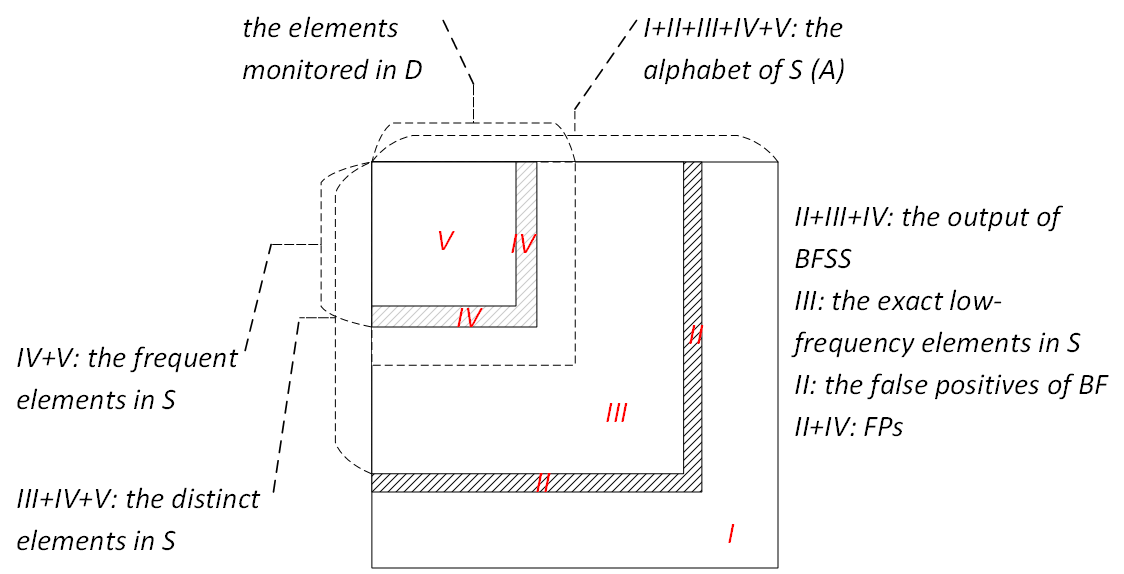
\includegraphics[width=2.8in]{png/bfss.png}
	\caption{Schematic diagram of the analysis of \emph{BFSS}}
	\label{fig:bfss}
\end{figure}

\subsubsection{\textbf{Analysis of FPs}}
In this section, we will give a theoretically strict bound of expectation of number of \emph{FPs} in output of \emph{BFSS} regardless of data distribution of $S$, and a tighter bound can be derived for data stream under Pareto distribution [].

\begin{lemma}\label{lem:6}
	 Any element $e$ with $f_S(e)>2\lfloor \phi N\rfloor$, must not be output.
\end{lemma}

\begin{IEEEproof}
From Lemma \ref{lem:4}, we know that any element $e$ with $f_S(e)>2\lfloor \phi N\rfloor$ must be monitored in $D$, i.e. $e\in E$. Then from Lemma \ref{lem:5}, we can get that elements monitored in $D$ must satisfy $f_S(e)\leq f(e)$, and that is to say any element $e$ monitored in $D$ with $f_S(e)>2\lfloor \phi N\rfloor$, must satisfy $f(e)>2\lfloor \phi N\rfloor$. At last from Lemma \ref{lem:3}, we can prove that any element $e$ with $f(e)>2\lfloor \phi N\rfloor$, must satisfy $f(e)>\lfloor \phi N\rfloor+\Delta(e)$, which means $e$ will not be output.
\end{IEEEproof}

\begin{lemma}\label{lem:7}
The probability of a false positive of \emph{BF} is no more than:
\begin{equation}
(1-(1-\frac{1}{K})^{HM})^H
\end{equation}
\end{lemma}

\begin{IEEEproof}
First, a false positive of \emph{BF} means an element in $A$ not appearing in $S$ but not filtered out by \emph{BF}. Observe that after inserting $M$ keys into a table of size $K$, the probability that a particular bit is still 0 is exactly
\begin{equation} 
(1-\frac{1}{K})^{HM}
\end{equation}
\indent Hence the probability of a false positive in this situation is $(1-(1-\frac{1}{K})^{HM})^H$. However, we know that $M$ denotes the size of $A$ which is the domain of $S$, so the number of distinct elements in $S$ must be no more than $M$, i.e. $M'\leq M$, and further we have $(1-(1-\frac{1}{K})^{HM'})^H\leq (1-(1-\frac{1}{K})^{HM})^H$.
\end{IEEEproof}

\begin{theorem}\label{thm:2}
Assuming no specific data distribution, the expectation of the number of \emph{FPs} in the output of \emph{BFSS}, denoted as $E(\#FPs)$, satisfies:
\begin{equation}\label{eq:7}
E(\#FPs)<M(1-(1-\frac{1}{K})^{HM})^H + \lceil\frac{1}{\phi}\rceil
\end{equation}
\end{theorem}

\begin{IEEEproof}
From Algorithm \ref{alg:bfss}, we can observe that two kinds of elements contribute to \emph{FPs}: i) the false positives of \emph{BF}; ii) the elements with $f_S(e)>\lfloor \phi N\rfloor$ wrongly output. The two cases correspond to the gray areas in Fig. \ref{fig:bfss} which is abstracted out from the analysis of \emph{BFSS}. Concretely speaking, the ligth gray area represents the elements with $f_S(e)>\lfloor \phi N\rfloor$ wrongly output, i.e. the second case, and the dark gray area represents the elements not filtered out by \emph{BF}, i.e. the first case. Furthermore, the output of \emph{BFSS} is represented by $II+III+IV$, and the exact low-frequency elements in $S$ is represented by $III$.\par
For the first case, we define the independent 0-1 random variables $x_i(1\leq i\leq M)$ for each element in $A$, and the value of $x_i$ depends on whether $a_i$ appeared in $S$ or not. If $a_i$ appeared in $S$, then $x_i=0$; If not, then with a probability of $(1-(1-\frac{1}{K})^{HM'})^H$, $x_i=1$; From the defination of $x_i$, we can find that the expectation of the number of the false positives of \emph{BF} equals $E(\sum_{i=1}^{M}x_i)$, i.e. $(M-M')(1-(1-\frac{1}{K})^{HM'})^H$.\par 
For the second case, we know from Lemma \ref{lem:6} that elements with $f_S(e)>2\lfloor \phi N\rfloor$ must not be not output, so only elements with $\lfloor \phi N\rfloor<f_S(e)\leq 2\lfloor \phi N\rfloor$ are likely to be output, and these elements must be monitored in $D$ which can be directly derived from Lemma \ref{lem:4}, so the maximum number of these elements is $\lceil\frac{1}{\phi}\rceil$. From above, due to the linear properties of expectation, we can get:
\begin{equation}\label{eq:8}
E(\#FPs)\leq (M-M')(1-(1-\frac{1}{K})^{HM'})^H+\lceil\frac{1}{\phi}\rceil\\
\end{equation}
\indent In addition, $M'\leq M$, so inequation \ref{eq:7} can be easily derived from inequation \ref{eq:8}.
\end{IEEEproof}

However, from the derivation above, we can see that $\frac{1}{\phi}$ is a loose bound of the second case because elements with $f_S(e)>2\lfloor \phi N\rfloor$ can not be output, and we count them in. So if we make an assumption of the distribution of $S$, we will get a relatively tighter bound of the second case.

\begin{theorem}\label{thm:3}
Assuming noiseless Pareto data with parameter $\alpha$ and $f_S(e_m)$, where $\alpha (\alpha >0)$ and $e_m$ denotes the element with the lowest freqeuncy, we have:
\setlength{\arraycolsep}{0.0em}
\begin{eqnarray}
	E(\#FPs)&<&M(1-(1-\frac{1}{K})^{HM})^H + T\\
	T&=&(\frac{f_S(e_m)}{\lfloor \phi N\rfloor})^\alpha(1-\frac{1}{2^\alpha})M\label{eq:10}
\end{eqnarray}
\setlength{\arraycolsep}{5pt}
\end{theorem}

\begin{IEEEproof}
The Pareto distribution has the following property: If $X$ is a random variable with a Pareto distribution, then the probability that $X$ is greater than some number $x$, i.e. the survival function is given by:
$$Pr(X>x)=
\begin{cases}
(\frac{x_m}{x}) & x\geq x_m\\
1 & x<x_m
\end{cases}$$
where $x_m$ is the minimum possible value of $X$, and $\alpha$ is a positive parameter. So In such a case, the expected value of the number of the elements with $\lfloor \phi N\rfloor<f_S(e)\leq 2\lfloor\phi N\rfloor$ is $(\frac{f_S(e_m)}{\lfloor \phi N\rfloor})^\alpha(1-\frac{1}{2^\alpha})M'$.
\end{IEEEproof}
We may not calculate the exact value of $T$ because we can't get the exact value of $f_S(e_m)$, however, once a query comes, the parameters are confirmed and so is the value of $T$, furthermore, the upper bound of the value of $E(\#FPs)$ is confirmed as well. In this sense, it is meaningful to give the expression of $T$.\par
From Inequation \ref{eq:7}, we observe that the upper bound of $E(\#FPs)$ is related with the values of $H$ and $K$, and our goal is to minimize the value of  $E(\#FPs)$ by choosing the appropriate values. In addtion, the value of $K$ directly influence the space complexity of \emph{BFSS}, so we will make some analysis of the values of $K$ and $H$ then.


\subsubsection{\textbf{Space complexity}}\label{sec:space}
In this section, we will give some analysis of the space complexity of \emph{BFSS} including how to choose the appropriate values of $H$ and $K$.

\textbf{Choosing the appropriate values of $H$ and $K$}. Our goal is to minimize $E(\#FPs)$, and from Algorithm \ref{alg:bfss}, we see that the values of $M$ and $\phi$ are confirmed at the very beginning before our algorithm. In this way, our task is to minimize the value of $(1-(1-\frac{1}{K})^{HM})^H$, denoted as $F$, by calculating the appropriate values of $H$ and $K$, and we have:
\begin{equation}\label{eq:11}
F\approx(1-e^{-\frac{HM}{K}})^H=e^{H\ln (1-e^{-\frac{HM}{K}})}
\end{equation}
Let $P=e^{-\frac{HM}{K}}$ and $G=H\ln (1-e^{-\frac{HM}{K}})$, and in order to minimize $F$, we only have to minimize $G$:
\begin{equation}\label{eq:12}
G=(-\frac{K}{M})\ln(P)\ln(1-P)
\end{equation}
The first derivative of $G$ with respect to $P$, denoted as $G'$, is:
\begin{equation}\label{eq:13}
G'=\frac{K}{M}(\frac{1}{1-P}\ln(P)-\frac{1}{P}\ln(1-P))
\end{equation}
From Equation \ref{eq:13}, we can easily observe that when $P=\frac{1}{2}$, $G$ reaches its minimum value. In this case, we have:
\begin{equation}\label{eq:14}
H=\frac{K}{M}\times\ln 2
\end{equation}
Combined with Equation \ref{eq:11} and Equation \ref{eq:14}, we have:
\begin{equation}\label{eq:15}
F\approx(1-e^{-\frac{HM}{K}})^H=(\frac{1}{2})^H\approx(0.6185)^{\frac{K}{M}}
\end{equation}
From the above derivation, we know that once the value of $\frac{K}{M}$ is confirmed, we can get the appropriate value of $H$ to minimize the value of $F$. For example, if the value of $\frac{K}{M}$ is set to 13, the appropriate value of $H$ is $\frac{K}{M}\times\ln 2\approx9.1$, because the value of $H$ is an integer, we set it to $9$. Considering the length limit, we give a small fraction of the value of $F$ under various $\frac{K}{M}$ and $H$ combinations in Table \ref{tab:2}.\par
\begin{table} 
	\centering
	\caption{The value of $F$ under various $\frac{K}{M}$ and $H$ combinations.}
   \begin{tabular}{|c|c|c|c|c|c|c|}
   	\hline
   	$K/M$ & $H$& $H=8$ & $H=9$ & $H=10$ & $H=11$ & $H=12$\\ 
   	\hline
   	13&9.01&0.00199&0.00194&0.00198&0.0021&0.0023\\
   	\hline
   	14&9.7&0.00129&0.00121&0.0012&0.00124&0.00132\\
   	\hline
   	15&10.4&0.000852&0.000775&0.000744&0.000747&0.000778\\
   	\hline
   	16&11.1&0.000574&0.000505&0.00047&0.000459&0.000466\\
   	\hline
   	17&11.8&0.000394&0.000335&0.000302&0.000287&0.000284\\
   	\hline
   \end{tabular}
    	\label{tab:2}
\end{table}
From Equation \ref{eq:15}, we notice that the larger the value of $H$ is, the smaller the value of $F$ is. However, the value of $K$ increases monotonically with the increasing value of $H$ once the value of $M$ is confirmed which can be observed from Equation \ref{eq:14}, in other words, in order to decrease the value of $E(\#FPs)$, we have to increase the size of \emph{BF}, i.e. $K$.\par 

For example, if the value of $M$ is 1M and the value of $\phi$ is 0.001. From Table \ref{tab:2}, we see that if the value of $K$ is 16M, the appropriate value of $H$ should be $11$, therefore the value of $F$ is 0.000459, and the upper bound of the value of $E(\#FPs)$ ,calculated by Inequation \ref{eq:7}, is $1M\times0.000459+1/0.001=1459$. Meanwhile, if the value of $K$ is 17M, the corresponding values of $H$ and $F$ are 12 and 0.000284, therefore the upper bound of the value of $E(\#FPs)$ is 1284. From the proof of Theorem \ref{thm:2}, we know that in order to caculate the exact upper bound of the value of $E(\#FPs)$, the bound given in Inequation \ref{eq:7} is not so tight, in fact, the experimental results indicate a much better performence.\par

\begin{theorem}\label{thm:4}
The space complexity of \emph{BFSS} is $O(\lambda M+ min(\lceil\frac{1}{\phi}\rceil,M))$, where $\lambda\in N^*$, the value of which is discussed detaily above. 
\end{theorem}

\begin{IEEEproof}
The space complexity of \emph{BFSS} includes two part: i) the size of \emph{BF}, i.e. $K$. ii) the number of counters used in $D$, i.e. $m$. In order to get the minimum value of $E(\#FPs)$, the value of $K$ should be multiple times of the value of $M$, i.e. $K=\lambda M(\lambda\in N^*)$. From Algorithm \ref{alg:output}, we have $m\leq min(\lceil\frac{1}{\phi}\rceil,M)$. So the space complexity of \emph{BFSS} is $O(\lambda M+ min(\lceil\frac{1}{\phi}\rceil,M))$.
\end{IEEEproof}

In conclusion, there exists a trade off between the number of \emph{FPs} and the space consumption of \emph{BFSS}. Theoretically, once the value of $M$ is confirmed, the larger the value of $\lambda$, the smaller the number of \emph{FPs} should be, and the larger the value of $K$ should be.\par
Furthermore, consider a naive method to solve $\phi$\emph{-Bounded Low-Frequency Elements}: we simply allocate each element in $A$ a counter, and update the corresponding counter for each element in $S$, when a query comes, we just output the elements with $f_S(e)\leq\lfloor \phi N\rfloor$. Obviously the method can maintain the low-frequency elements precisely, and the space complexity of the method is $O(M)$. \emph{BFSS} has no advantage over the naive method in space complexity considering big O though, \emph{BFSS} needs not to store the exact value or the fingerprint of each element which may consume much space in total especially when the value is long string, URL etc. The experimental results indicate \emph{BFSS} is much more space efficient too.
\subsubsection{\textbf{Time complexity}}
In this section, we will discuss the time complexity of \emph{BFSS}.

\begin{theorem}\label{thm:5}
Processing each data stream element needs $O(1)$ time, independent of the size of the stream.
\end{theorem}

\begin{IEEEproof}
From Algorithm \ref{alg:bfss}, we know the processing time for each element consists two parts: i) the time spent hasing each element into \emph{BF}. ii) the time spent updating the corresponding counter in $D$. Due to $H$ is constant, time spent hashing each element into \emph{BF} is constant too. Consider two cases in updating the corresponding counter in $D$: i) element $e$ is monitored in $D$, and we only have to update the corresponding counter. ii) element $e$ is not monitored in $D$, and we need to first locate the counter with the minimum $f(e)$, then update it. Obviously, the time spent for any case is constant because $\lceil \frac{1}{\phi}\rceil$ is constant. Therefore, processing each element needs only $O(1)$ time in total.
\end{IEEEproof}

\subsubsection{\textbf{Challenges to BFSS}}
In this section, we will identify the existing problems in \emph{BFSS}.\par
From the analysis in section \ref{sec:space} , we observe that $K$ should increase monotonically with $M$ in order to keep a low rate of \emph{FPs}, however, what if $M$ is extremely large? Consider such a case: if $M=4G$, i.e. 4 billion, and in order to keep $F$ less than 0.05\%, we have to set $K=64G$, i.e the space used by \emph{BF} is 8GB, which may exceed the memory limit of a normal PC.\par
Inspired by the algorithm proposed in [], we present the \emph{SBFSS} algorithm, which can find low-frequency elements over the data streams from extremely large domain with acceptable number of \emph{FPs} and \emph{FNs} using proper space.\par

\subsection{The SBFSS Algorithm}\label{sec:sbfss}
In this section, we will introduce the \emph{SBFSS} algorithm, which improve the \emph{BFSS} algorithm and can handle the data streams from large domain.\par
The major difference between \emph{BFSS} and \emph{SBFSS} is the Bloom filter we use. Concretely speaking, \emph{BF} is a regular Bloom filter, while \emph{SBF} change bits in \emph{BF} into cells, each consisting of one or more bits. In addition, from the explaination above, the size of \emph{BF}, i.e. $K$, should increase monotonically with $M$, however, there can be no linear relationship between the size of \emph{SBF}, i.e. $K'$, and $M$, and $K'$ can be any integer predefined by users. Defination \ref{def:1} is the detailed defination of \emph{SBF}.\par  

\newtheorem{defn}{Definition}
\begin{defn}\label{def:1}
\emph{SBF} is defined as an array of integer $SBF[1],SBF[2],...,SBF[k]$ whose minimum value is 0 and maximum value is $max$. Each element of the array is allocated $d$ bits. The relation between $max$ and $d$ is then $max=2^d-1$. Compared to bits in a regular Bloom filter, each element of the \emph{SBF} is called a cell.
\end{defn}

Like \emph{BFSS}, \emph{SBFSS} consists of two phases: updating and quering. Algorithm \ref{alg:sbfss} and Algorithm \ref{alg:soutput} give the detailed descriptions of them.   Because of the limitation of length, no more tautology here.

\begin{algorithm}[h]
	\caption{SBFSS Update Algorithm}
	\label{alg:sbfss}
	\begin{algorithmic}[1]
		\REQUIRE Stream $S$, support threshold $\phi$
		\STATE The form of the counters in $D$ is $(e,f(e),\Delta(e))$
		\FOR{$i=0$ to $k-1$}
		\STATE $SBF[i]=0$
		\ENDFOR
		\FOR{each item $e$ of stream $S$}
		\STATE Select $P$ different cells uniformly at random $SBF[j_1]...SBF[j_P]$, $P\in \{1,...,k\}$
		\FOR{each cell $SBF[j]\in\{SBF[j_1]...SBF[j_P]\}$}
		\IF{$SBF[j]\geq 1$}
		\STATE $SBF[j]=SBF[j]-1$
		\ENDIF
		\ENDFOR
	    \FOR{$i=1$ to $H$}
		\STATE $SBF[h_i(e)]=max$
		\ENDFOR
		\IF{$e$ is monitored in $D$}
		\STATE $f(e)=f(e)+1$;
		\ELSIF{$m<C$}
		\STATE Assign a new counter $(e,1,0)$ to it
		\STATE $m=m+1$
		\ELSE
		\STATE Let $e_m$ be the element with least hits, $min$
		\STATE Replace $e_m$ with $e$ in $D$
		\STATE $f(e)=min+1,\Delta(e)=min$
		\ENDIF
		\STATE $N=N+1$;
		\ENDFOR
	\end{algorithmic}
\end{algorithm}

\begin{algorithm}[h]
	\caption{SBFSS Query Algorithm}
	\label{alg:soutput}
	\begin{algorithmic}[1]
		\REQUIRE \emph{SBF}, $D$, $\phi$, $A$, $N$, $M$
		\ENSURE low-frequency elements with threshold $\phi$
		\STATE $flag=true$; \COMMENT{ \emph{flag}: indicate whether an element is in \emph{SBF} or not}
		\FOR{$i=0$ to $M-1$}
		\STATE $flag=true$
		\FOR{$j=1$ to $H$}
		\IF{$SBF[h_j(A[i])]==0$}
		\STATE $flag=false$
		\STATE break;
		\ENDIF
		\ENDFOR
		\IF{$flag==true$}
		\IF{$A[i]$ is monitored in $D$}
		\IF{$f(A[i])\leq\lfloor \phi N\rfloor+\Delta(A[i])$}
		\STATE output $A[i]$ as a low-frequency element
		\ENDIF
		\ELSE
		\STATE output $A[i]$ as a low-frequency element
		\ENDIF
		\ENDIF
		\ENDFOR
	\end{algorithmic}
\end{algorithm}

From Algorithm \ref{alg:sbfss}, we observe that there are two kinds of operation on \emph{SBF}. First randomly decrement $P$ cells by 1 so as to make room for fresh elements
; then set the same $H$ cells as in the update process to $max$.\par 
Intuitively, due to the random deletion operation, \emph{SBF} does not exceed its capacity in a data stream scenario, however, false negatives may come up as well.

\subsection{Analysis of SBFSS}
Like \emph{BFSS}, we will give theoretical analysis of \emph{SBFSS} in this section, including the equivalence of \emph{SBF'} (the \emph{SBF} used in []) and \emph{SBF}, \emph{FNs}, \emph{FPs}, parameters setting, and time complexity.\par
\subsubsection{\textbf{Analysis of the equivalence of SBF' and SBF}}
\emph{SBF'} is used to detect duplicates over data streams, in fact, from Algorithm \ref{alg:sbfss} and Algorithm \ref{alg:soutput}, we can observe that \emph{SBF} is used to filter out the elements that never appeared in $S$, and we check whether the element in $A$ is duplicated one by one, if the element is a duplicate, we just claim it appeared in $S$, in this sense, \emph{SBF'} and \emph{SBF} share the same function. So the properties of \emph{SBF'}, including the probability of a false positive and a false negative of \emph{SBF'}, are fully applicable to \emph{SBF}.\par

\subsubsection{\textbf{Analysis of FPs}}
In this section, we will give a theoretically upper bound of the expectation of the number of \emph{FPs} in the ouput of \emph{SBFSS}.\par
The detailed proof of Lemma \ref{lem:8} can be found in []. Because of the limitation of length, no more tautology here.
\begin{lemma}\label{lem:8}
The probability of a false positive (FP) of \emph{SBF} is no greater than :
\begin{equation}
(1-(\frac{1}{1+\frac{1}{P(1/H-1/m)}})^{max})^H
\end{equation}
\end{lemma}

\begin{theorem}\label{thm:6}
Assuming no specific data distribution, the expectation of the number of \emph{FPs} in the output of \emph{SBFSS}, denoted as $E'(\#FPs)$, satisfies:
\begin{eqnarray}\label{eq:17}
E'(\#FPs)<M \min \{(1-(\frac{1}{1+\frac{1}{P(1/H-1/m)}})^{max})^H,\\\nonumber
	(1-(1-\frac{1}{k})^{HM})^H\} + \lceil\frac{1}{\phi}\rceil
\end{eqnarray}
\end{theorem}

\begin{IEEEproof}
From Fig. \ref{fig:sbfss}, we notice that the \emph{FPs} of \emph{SBFSS} has two parts: i) the false positives of \emph{SBF}, i.e. $II$; ii) the elements with $f_S(e)>\lfloor\phi N\rfloor$ wrongly output, i.e. $VI$. In fact, $V$ is the only difference between the \emph{FPs} of \emph{SBFSS} and the \emph{FPs} of \emph{BFSS}, for \emph{BFSS}, the elements in $V$ will be output, however, due to the false negatives of \emph{SBF} in \emph{SBFSS}, i.e. $IV+V+VIII$, the elements in $V$ will be neglected by \emph{SBFSS}, in this sense, the false negatives of \emph{SBF} inversely reduce the number of \emph{FPs} of \emph{SBFSS}. \par
In fact, the posibility of a false positive of \emph{SBF} must be smaller than that of \emph{BF} under the same conditions because \emph{SBF} brings in decrement operation. For the first case, we can get the upper bound of the expectation of the number of the false positives of \emph{SBF} through Lemma \ref{lem:7} and Lemma \ref{lem:8}. For the second case, it is clearly to see from Fig. \ref{fig:sbfss} that the maximum of the area of $VI$ is $\lceil\frac{1}{\phi}\rceil$, which is the area of the square surrounded by dotted lines, and obviously it is a loose bound. The residual derivation is obvious and exactly the same as Theorem \ref{thm:2}, and no more tautology here.
\end{IEEEproof}
Like \emph{BFSS}, a tighter bound of the area of $VI$ can be obtained if we assume the distribution of $S$, and the bound is $(\frac{f_S(e_m)}{\lfloor \phi N\rfloor})^\alpha(1-\frac{1}{2^\alpha})M$, the derivation of which is exactly the same as E.q. \ref{eq:10}, if the distribution is Pareto. In addition, due to the exsitence of $V$, the number of the elemens with $f_S(e)>\lfloor\phi N\rfloor$ wrongly output is smaller than that of \emph{BFSS} regardless of the data distribution of $S$. 
\begin{figure}
	\centering
	\includegraphics[width=2.8in]{png/sbfss.png}
	\caption{Schematic diagram of the analysis of \emph{SBFSS}}
	\label{fig:sbfss}
\end{figure}

\subsubsection{\textbf{Analysis of FNs}}
In this section, unlike \emph{BFSS}, we will give a theoretically upper bound of the expectation of the number of \emph{FNs} in the ouput of \emph{SBFSS}. \par
From Fig. \ref{alg:sbfss}, we can see that the \emph{FNs} of \emph{SBFSS}, $IV$, is a portion of the false negatives of \emph{SBF}, $IV+V+VIII$. Therefore the upper bound of the number of \emph{FNs} in the output of \emph{SBFSS} is the number of the false negatives of \emph{SBF}.\par
First, let us consider the probability of a false negative of \emph{SBF} which is an error when an element in $S$ wrongly filtered out by \emph{SBF}. Therefore only the elements in $S$ can generate false negatives, obviously the number of false negatives is related to the input data distribution.\par
Suppose an element $A[i]$ appearing in $S$ whose last appearence in $S$ before a query comes is $e_{i-\delta_i}$, where $\delta_i$ represents the number of elements in $S$ during the time between the last appearance of $A[i]$ and a query, is hashed into $H$ cells, $SBF[C_{i1}],...,SBF[C_{iH}]$. A false negative happens if any of those $H$ cells is decremented to 0 during the $\delta_i$ iterations when a query comes. Let $PR_0(\delta_i,p'_{ij})$ be the probability that cell $C_{ij} (j = 1...H)$ is decremented to 0 within the $\delta_i$ iterations, and $A_l$ denotes the event that within the $N$ iterations the most recent setting operation applied to the cell occurs at iteration $N-l$, and $A'_N$ denotes the event that cell has never been set within the whole $N$ iterations. $PR_0(\delta_i,p'_{ij})$ can be computed as:
\begin{equation}\label{eq:18}
\begin{split}
PR_0(\delta_i,p'_{ij})=\sum_{l=max}^{\delta_i-1}[Pr(SBF_{\delta_i}=0|A_l)Pr(A_l)]\\
+Pr(SBF_{\delta_i}=0|A_{\delta_i})Pr(A'_{\delta_i})
\end{split}
\end{equation}
where 
\setlength{\arraycolsep}{0.0em}
\begin{eqnarray}\label{eq:19}
Pr(SBF_{\delta_i}=0|A_l)&=&\sum_{j=max}^{l}\left(^l_j\right)p^j(1-p)^{l-j}\\
Pr(A_l)&=&(1-p'_{ij})^lp'_{ij}\\
Pr(SBF_{\delta_i}=0|A'_{\delta_i})&=&\sum_{j=max}^{\delta_i}\left(^{\delta_i}_j\right)p^j(1-p)^{\delta_i-j}\\
Pr(A'_{\delta_i})&=&(1-p'_{ij})^{\delta_i}
\end{eqnarray}
\setlength{\arraycolsep}{5pt}
Based on E.q \ref{eq:18}, the expected value of the false negatives of \emph{SBF}, $E(\#FN)$, can be easily derived, and the tailed derivation of E.q \ref{eq:18} and Lemma \ref{lem:9} can be found in [], therefore no more tautology here.\par

\begin{lemma}\label{lem:9}
There must be an "average" $\widehat{\delta}$ and an "average" $\widehat{p'}$ such that: 
\begin{equation}\label{eq:20}
E(\#FN)=M'[1-(1-PR_0(\widehat{\delta},\widehat{p'}))^H]
\end{equation}
\end{lemma}

\begin{theorem}\label{thm:7}
	Assuming no specific data distribution, the expectation of the number of \emph{FNs} in the output of \emph{SBFSS}, denoted as $E'(\#FNs)$, satisfies:
	\begin{equation}\label{eq:24}
	E'(\#FNs)\leq M[1-(1-PR_0(\widehat{\delta},\widehat{p'}))^H]
	\end{equation}
\end{theorem}

\begin{IEEEproof}
Like \emph{FPs}, two kinds of elements contribute to \emph{FNs}: i) the elemtents with $0<f_S(e)\leq\lfloor \phi N\rfloor$ wrongly filtered out by \emph{SBF}; ii) the elemtents with $f_S(e)\leq\lfloor \phi N\rfloor$ monitored in $D$ wrongly neglected. In fact, elements with $f_S(e)\leq\lfloor \phi N\rfloor$ must satisfy $f(e)\leq\lfloor \phi N\rfloor+\Delta(e)$, which means no elements with $f_S(e)\leq\lfloor \phi N\rfloor$ monitored in $D$ wrongly neglected. For the first case, we assume that the false negatives are all elements with $0<f_S(e)\leq\lfloor \phi N\rfloor$, i.e. neglecting $V+VIII$ in Fig. \ref{fig:sbfss}, which is the worst case, and in this way we have $E(\#FN)=E(\#FNs)=M'[1-(1-PR_0(\widehat{\delta},\widehat{p'}))^H]\leq M[1-(1-PR_0(\widehat{\delta},\widehat{p'}))^H]$.
\end{IEEEproof}
From E.q \ref{eq:17}, we observe that the upper bound of $E'(\#FPs)$ is completely related to \emph{SBF} once the parameter $\phi$ is confirmed, and the upper bound of $E'(\#FNs)$ is totally related to \emph{SBF} which can be observed from E.q \ref{eq:24}. In this way, we will give some analysis of how to choose appropriate parameters of \emph{SBF} next.

\subsubsection{\textbf{Parameters setting}}
In this section, we will discuss how to choose appropriate parameters of \emph{SBF} in \emph{SBFSS}.\par 
For \emph{SBFSS}, users will specify $\phi$, $\#FPs$ and memory limit $L$. The memory consumption of \emph{SBFSS} mainly contains two parts: \emph{SBF} and $D$. From Algorithm \ref{alg:sbfss}, we know that there are at most $\lceil\frac{1}{\phi}\rceil$ counters in $D$, and in this way we can estimate the memory available for \emph{SBF}, and through E.q \ref{eq:17}, we can estimate the FP rate, in fact, the FP rate can be a little larger than the caculated one beacause only a part of elements cause false positives. Therefore our goal is to choose a combination of $max,H$ and $P$ that minimizes the number of FNs under the condition that the FP rate is within a confirmed threshold and a fix amount of space.\par
In fact, a detailed discussion of how to choose these parameters has been given in [], which can concluded as: A formula can be obtained to compute the value of $P$ from other parameters provided that $max$ and $H$ have been chosen already; then find the optimal values of $H$ for each case of $max(1,3,7)$ by trying limited number$(\leq 10)$ of values of $H$ on the FN rate formulas; Last, $max$ can be set empirically, and specially in the case that no prior knowledge of the input data is available, [] suggests setting $max=1$.

\subsubsection{\textbf{Time complexity}}
In this section, we will analyze the time complexity of \emph{SBFSS}.\par
For \emph{SBFSS}, the amount of space has been confirmed, so we just focus on time complexity.

\begin{theorem}\label{thm:8}
For \emph{SBFSS}, Processing each data stream element needs $O(1)$ time, independent of the size of space and the stream.
\end{theorem}

\begin{IEEEproof}
Like \emph{BFSS}, the processing time for each element also consists two parts: i) the time spent updating \emph{SBF}; ii) the time spent updating $D$. In fact, from Algorithm \ref{alg:bfss} and Algorithm \ref{alg:sbfss}, we can see that \emph{BFSS} and \emph{SBFSS} share the same operations on $D$, so for \emph{SBFSS}, the time spent updating $D$ is constant once $\phi$ is confirmed, which means the size of space has no impact on it. For the first part, a detailed explaination has been given in [] to prove that the time spent updating \emph{SBF} is O(1), independent of the size of space and the stream. Therefore the time complexity of \emph{SBFSS} is O(1).
\end{IEEEproof}


\section{Experiments}
In this section, we first describe our data sets and the implementation details of \emph{BFSS} and \emph{SBFSS}, then we tested the performance of \emph{BFSS} under different parameter settings on both real and synthetic data sets, then we compared the results against the method \emph{nCount} and the method \emph{rCount}. We were insterested in the \emph{recall}, the number of correct elements found as a percentage of the number of correct elements; and the \emph{precision}, the number of correct elements found as a percentage of the entire output. We also measured the space used by \emph{BFSS} and \emph{nCount}, which is essential to handle data streams. For \emph{SBFSS}, we compared the recall and precision against the method \emph{lCount} in limited space of different size on real data sets. The detailed implementations of \emph{nCount}, \emph{rCount} and \emph{lCount} will be given later. Last, we give a summarization of the experimental results. All the algorithms were compiled using the same compiler, and were run on a AMD Opteron(tm) 2.20GHz PC, with 64GB RAM, and 1.8TB Hard disk.\par
\begin{figure*}[!t]
	\begin{minipage}{0.3\linewidth}
		\centering
		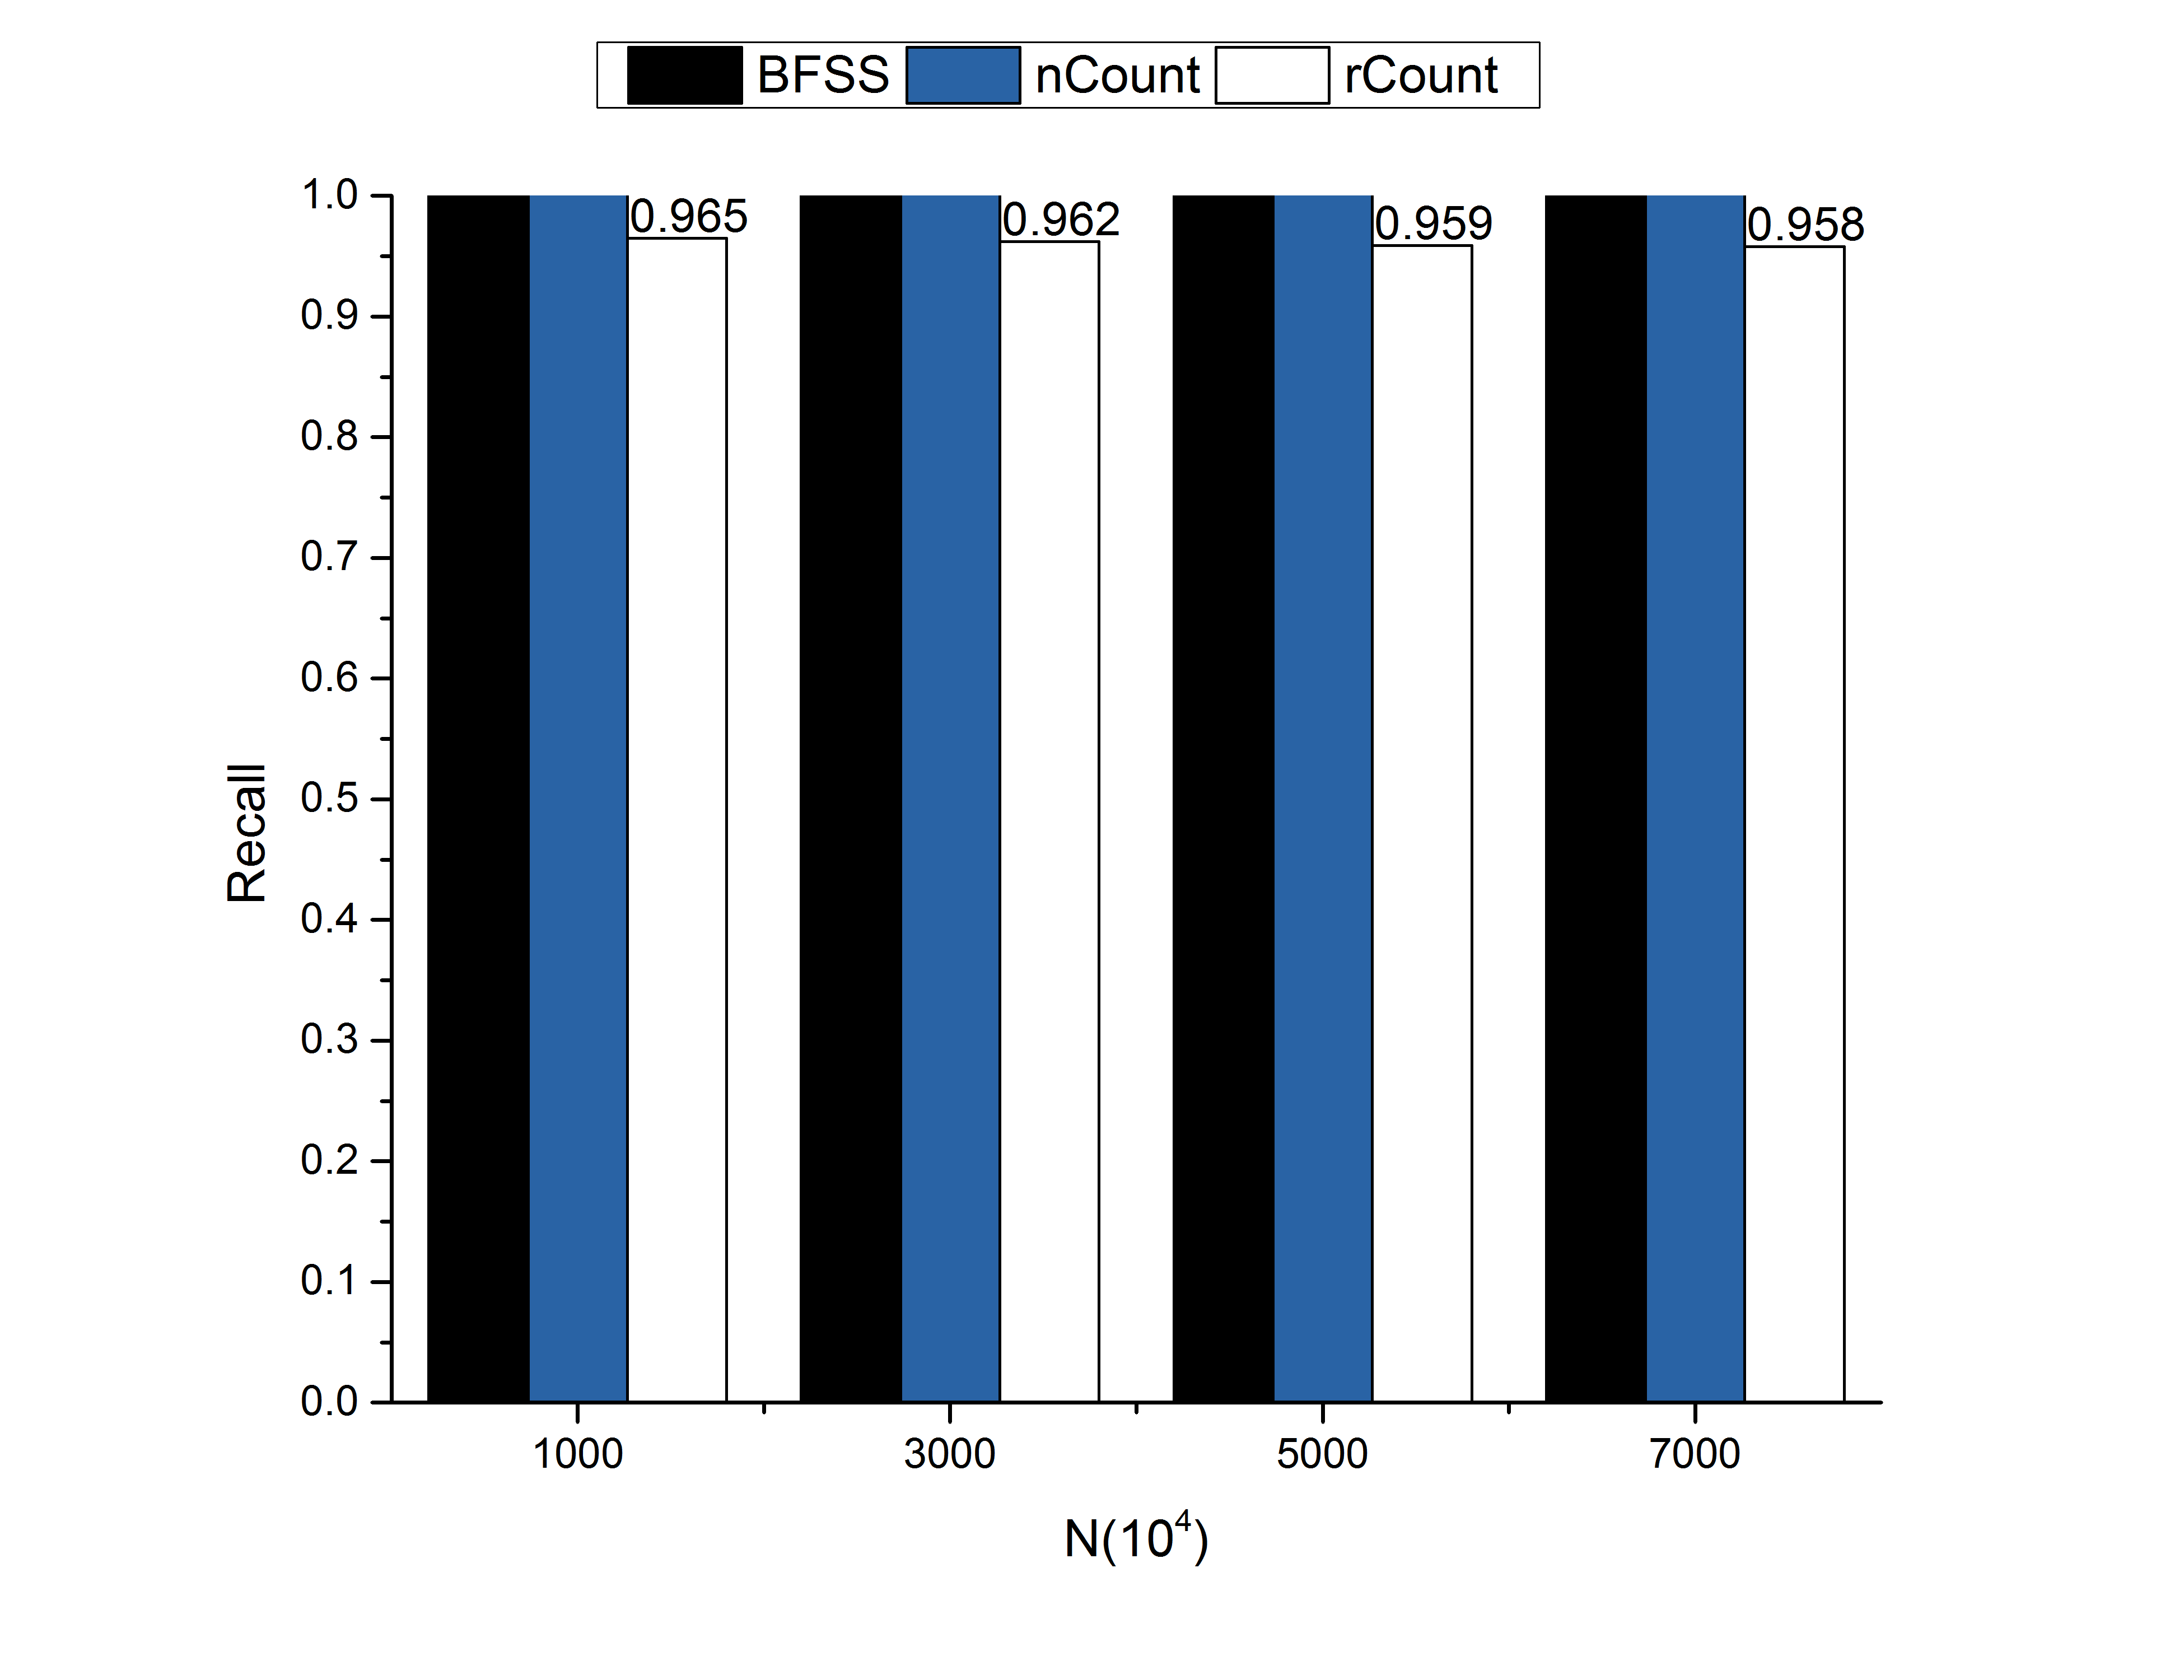
\includegraphics[width=2.8in]{png/zipf-recall.png}
	\end{minipage}
	\begin{minipage}{0.3\linewidth}
		\centering
		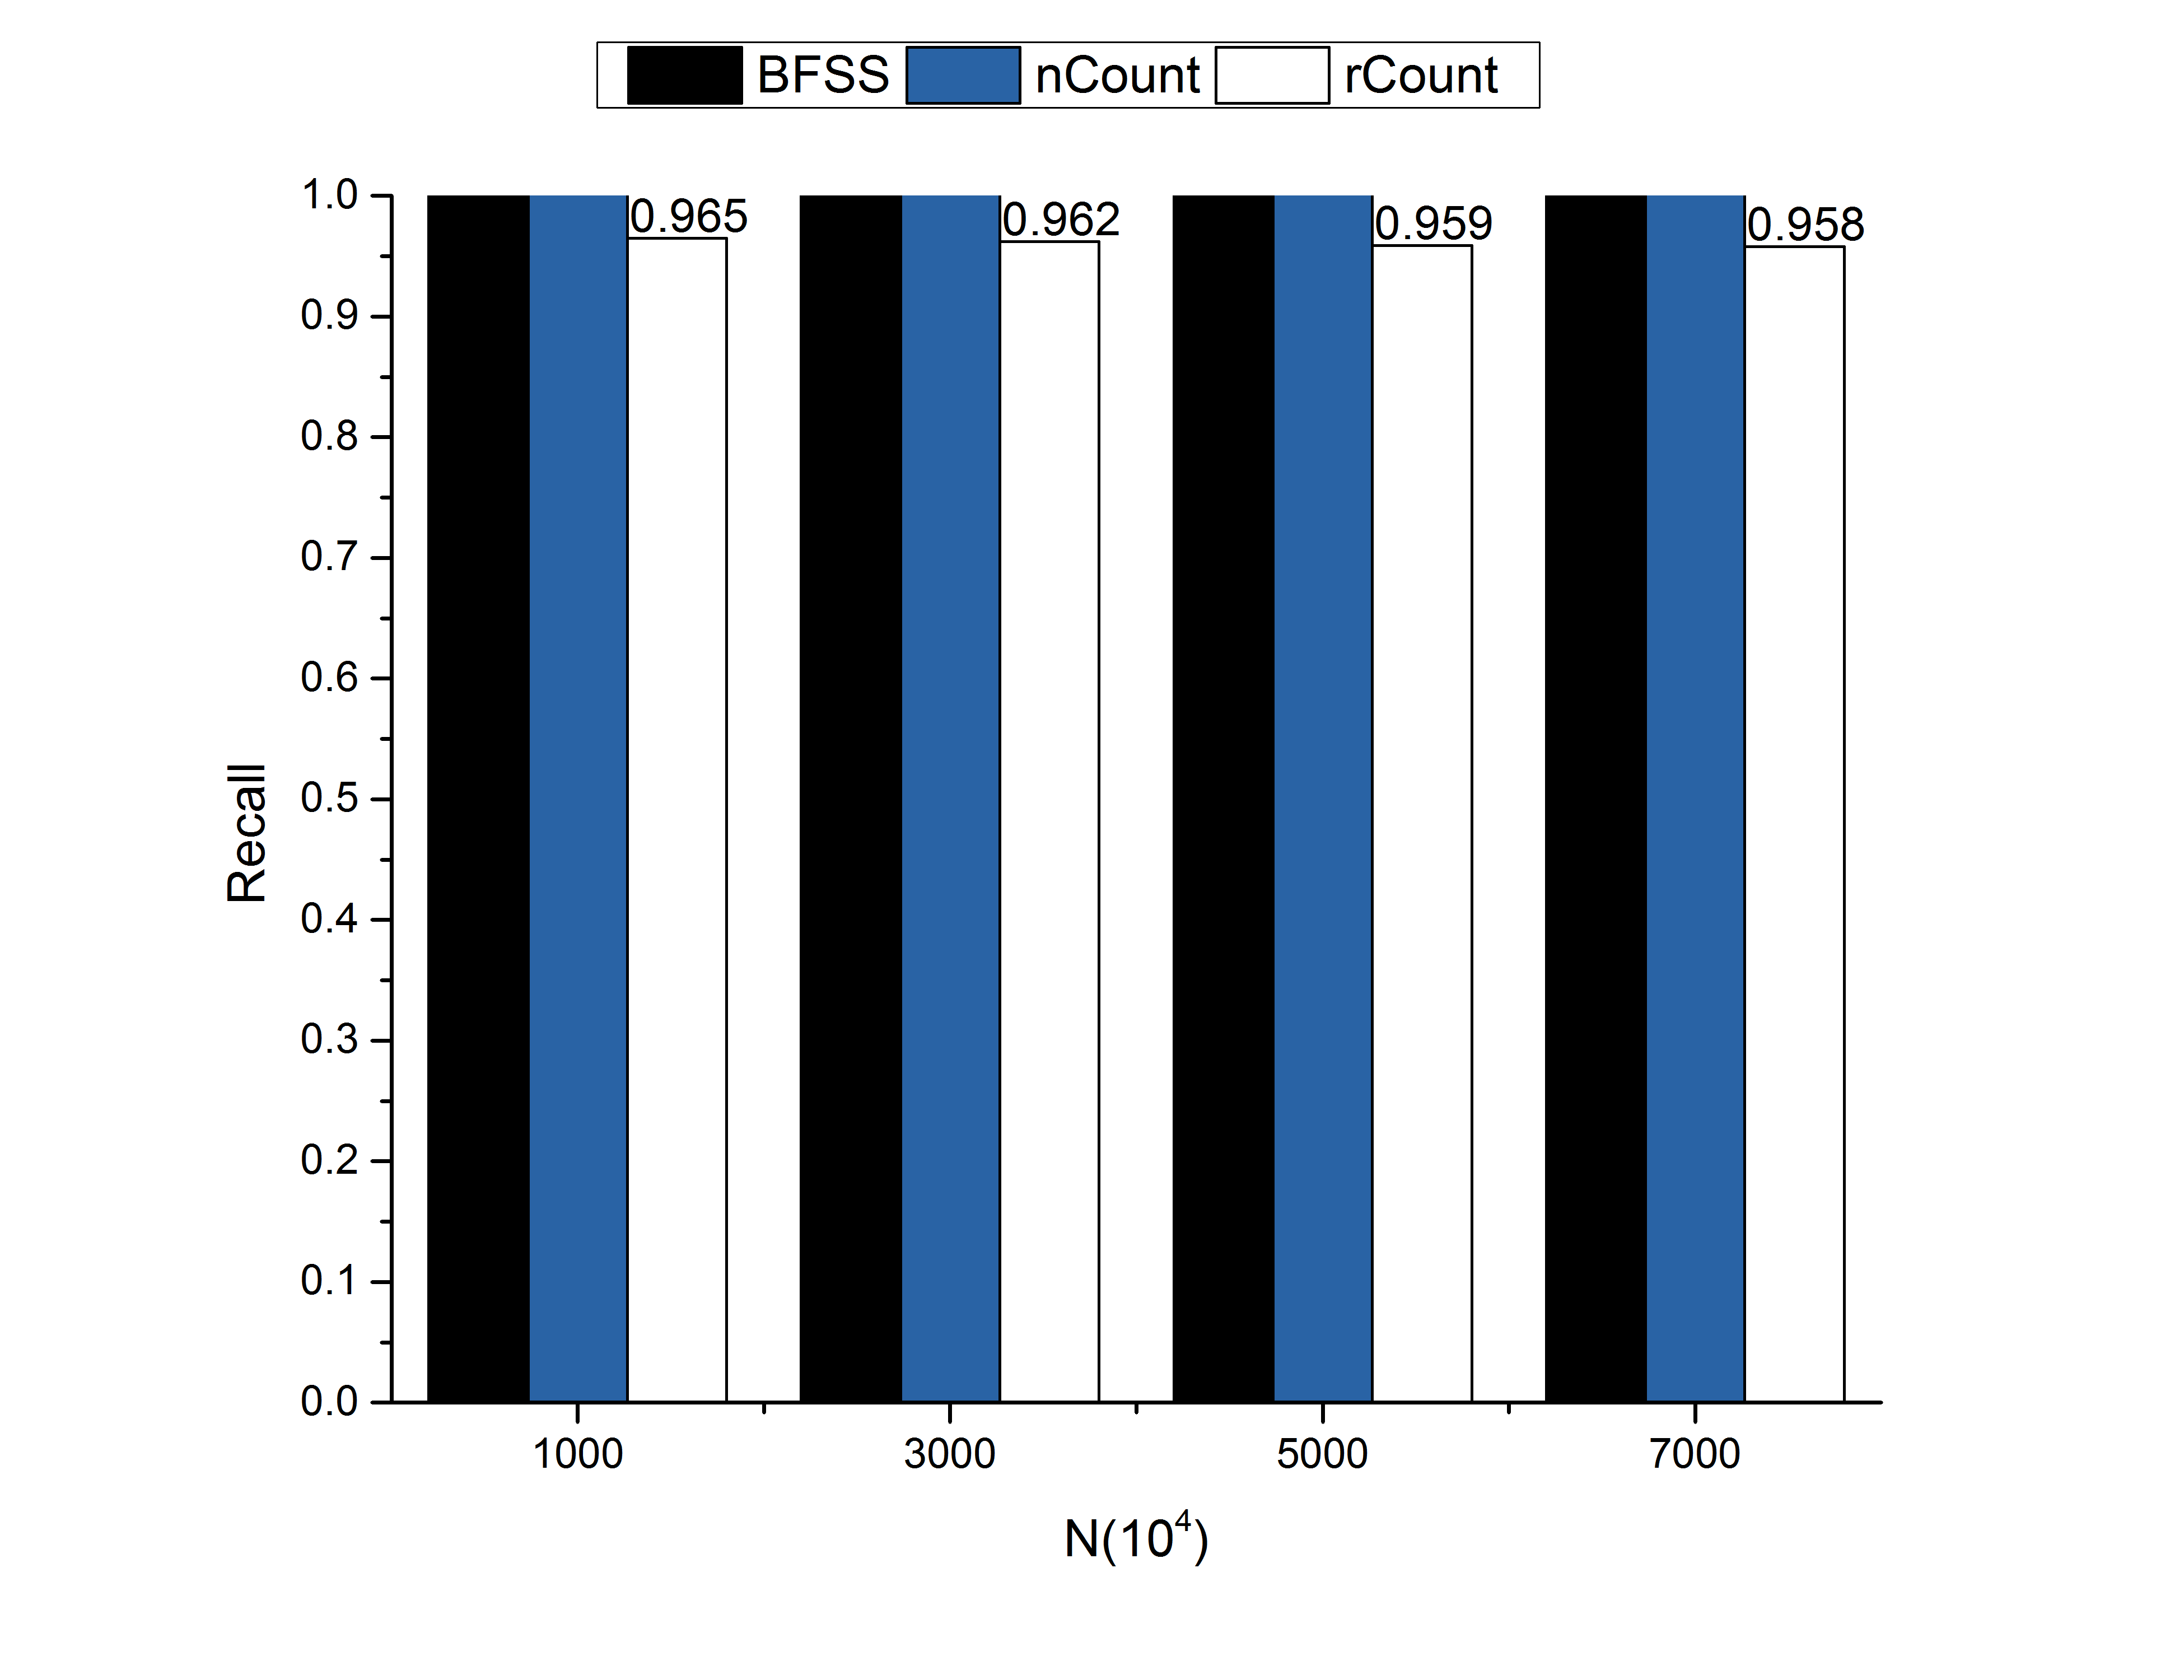
\includegraphics[width=2.8in]{png/zipf-recall.png}
	\end{minipage}
	\begin{minipage}{0.3\linewidth}
		\centering
		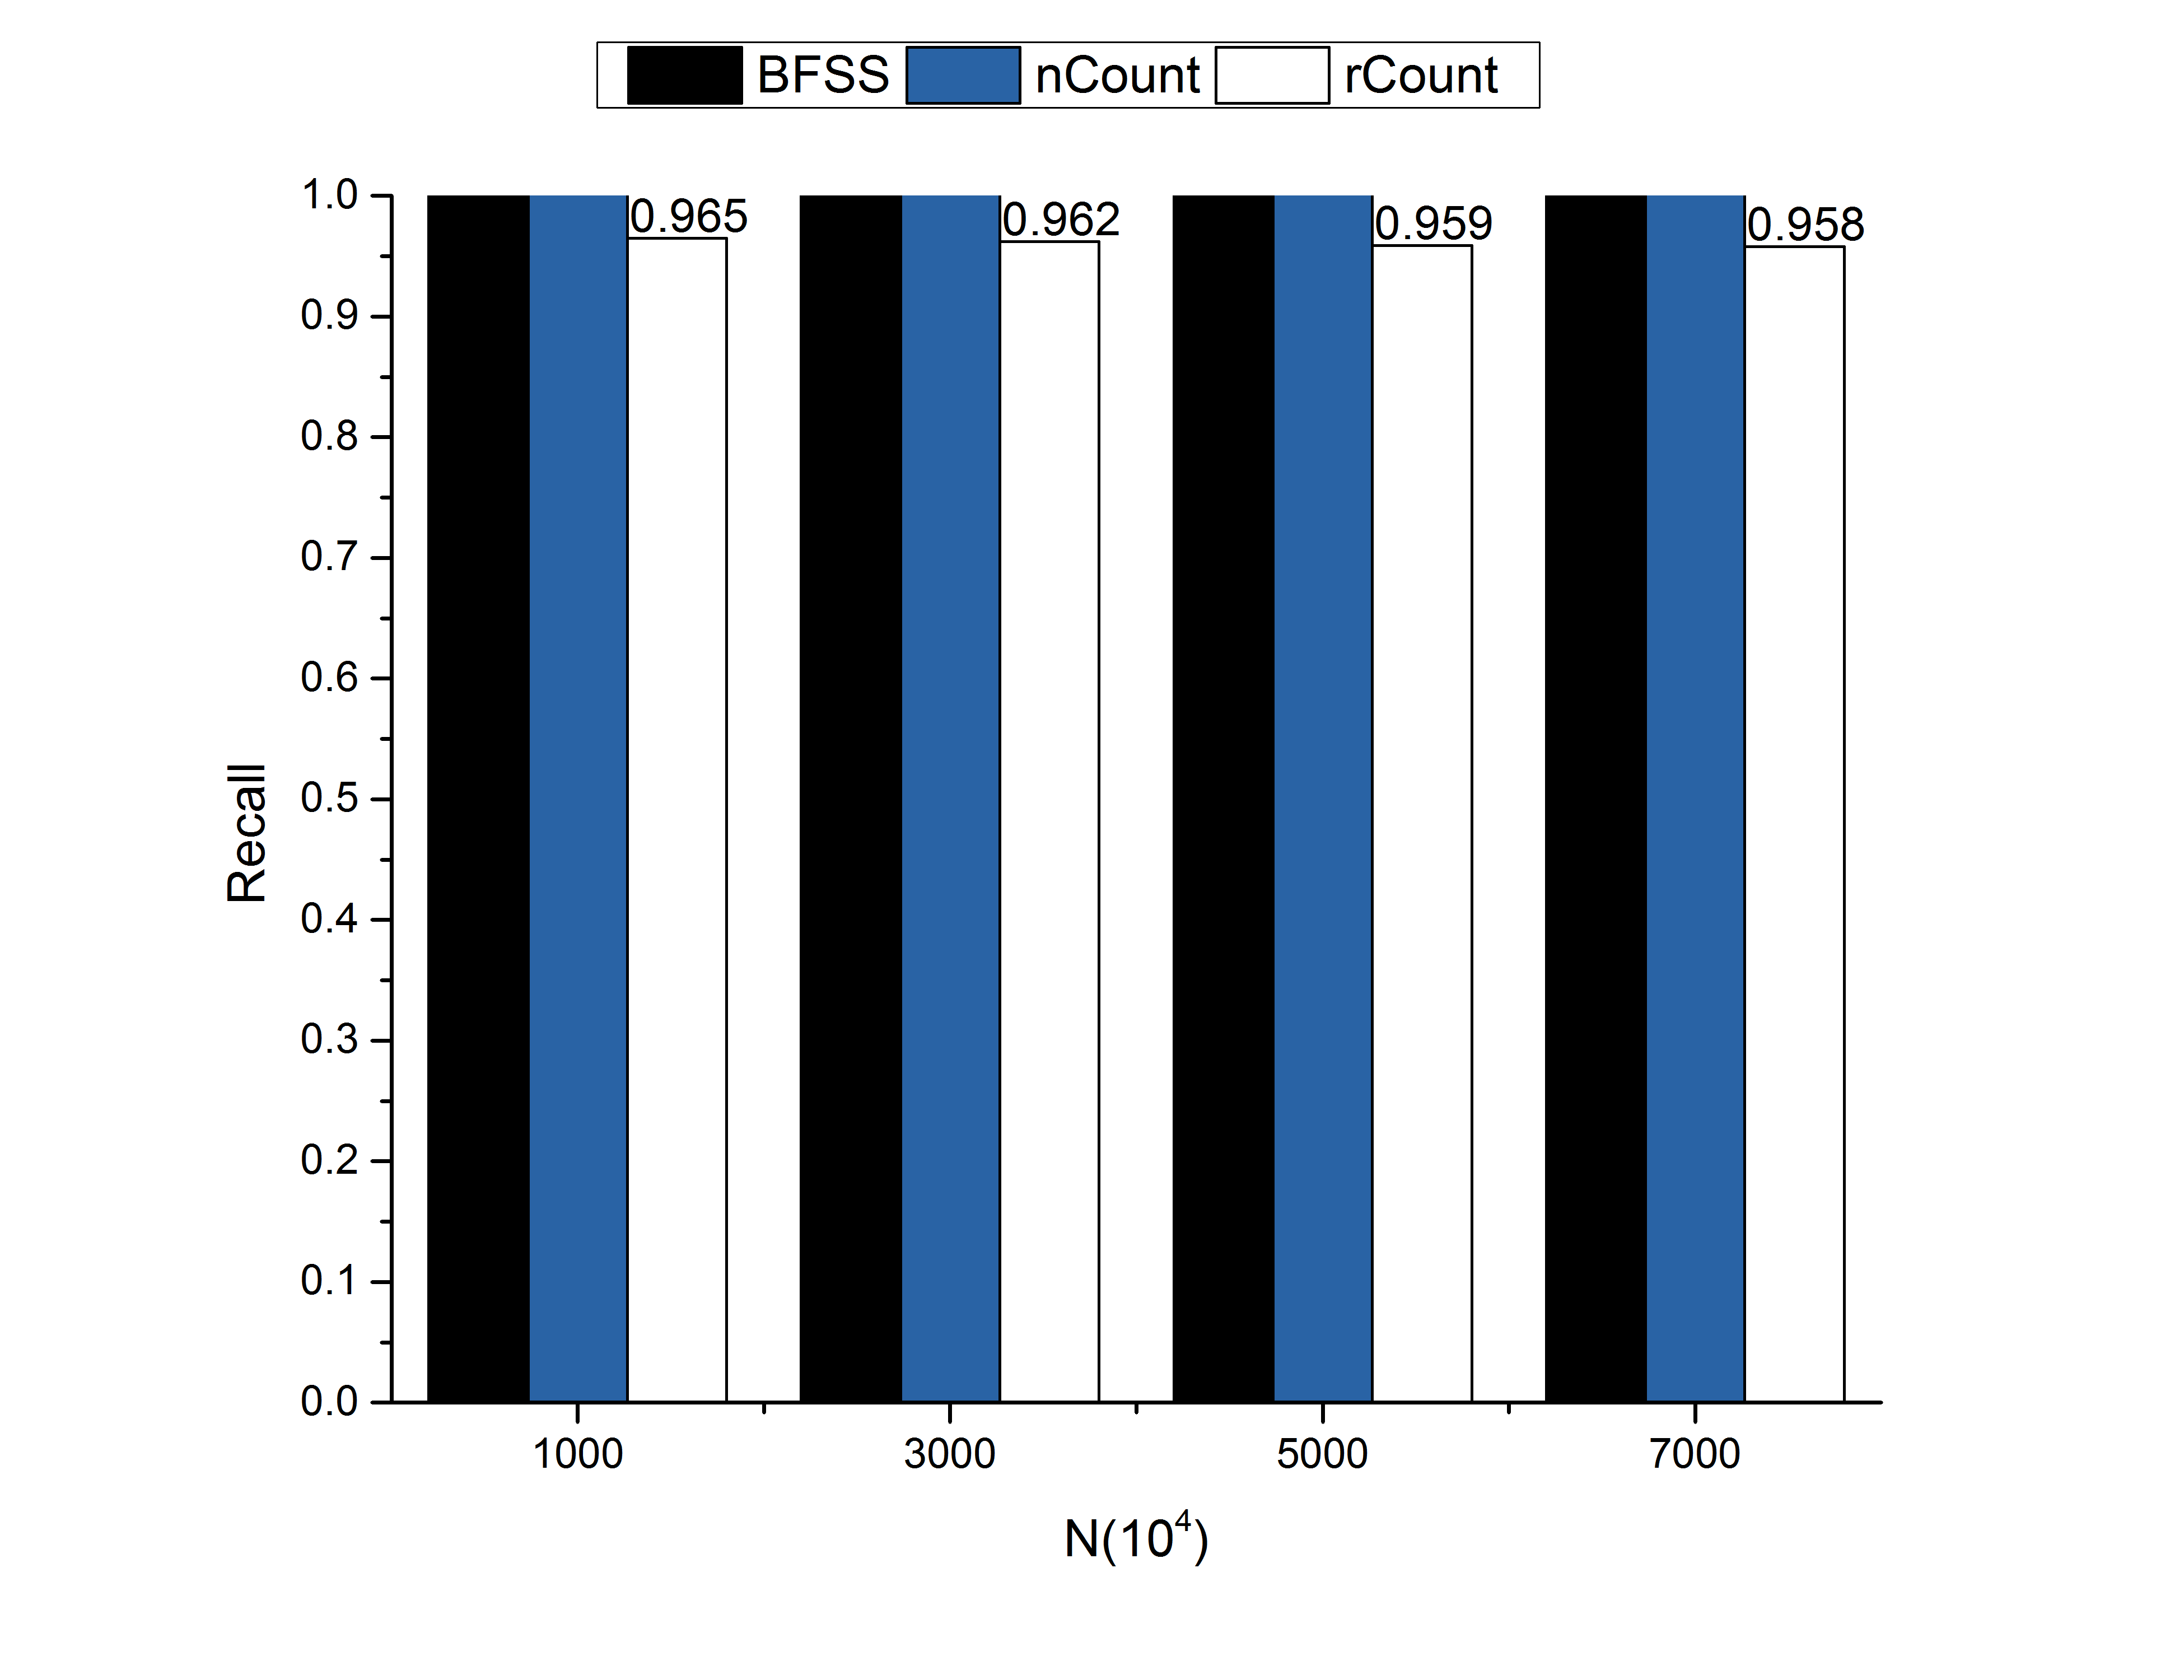
\includegraphics[width=2.8in]{png/zipf-recall.png}
	\end{minipage}
	\caption{Schematic diagram of the analysis of \emph{SBFSS}}
	\label{fig:zipf-recall}
\end{figure*}

\begin{table*}[!t] 
\centering 
\caption{Network Delay as a Function of Load} 
\label{table_delay} 
\begin{IEEEeqnarraybox}[\IEEEeqnarraystrutmode\IEEEeqnarraystrutsizeadd{2pt}{0pt}]{x/r/Vx/r/v/r/x}
\IEEEeqnarraydblrulerowcut\\ 
&&&&\IEEEeqnarraymulticol{3}{t}{Precision}&\\ &\hfill\raisebox{-3pt}[0pt][0pt]{$\beta$}\hfill&&\IEEEeqnarraymulticol{5}{h}{}%
\IEEEeqnarraystrutsize{0pt}{0pt}\\ 
&&&&\hfill0.1\hfill&&\hfill 0.01\hfill&\IEEEeqnarraystrutsizeadd{0pt}{2pt}\\ \IEEEeqnarraydblrulerowcut\\ 
&1&&& 0.057&& 0.172&\\ 
&10&&& 0.124&& 0.536&\\ 
&100&&& 0.830&& 0.905\rlap{\textsuperscript{*}}&\\ 
\IEEEeqnarraydblrulerowcut\\ 

\end{IEEEeqnarraybox} 
\end{table*} 


\subsection{Data Sets}
\textbf{Real Data.} For real data experiments, we used the dataset which consists of all the requests made to the 1998 World Cup Web site between April 30, 1998 and July 26, 1998 []. We extracted $7\times10^7$ URLs in total.\par
\textbf{Synthetic Data.} We generated several synthetic Zipfian data sets with the Zipf parameter varying from 0.5, which is very slightly uniform, to 3.0, which is highly skewed, with a fixed increment of 0.5. The size of each data set, N, is $10^7$, and the alphabet was of size $10^6$.
\subsection{Implementation Issues}
\textbf{\emph{BFSS} Implementation.} It is simple and straight forward to implement \emph{BFSS}: 1) hash each incoming stream element into $H$ numbers, and set the corresponding $H$ bits to 1. 2) we maintain a min heap to index each counter in $D$, if there exists an empty counter, we just insert a new counter into the heap, otherwise we replace the top counter of the heap, at last we readjust the heap. 3) when a query comes, we just do as Algorithm \ref{alg:output} indicates.\par

\textbf{\emph{SBFSS} Implementation.} The only difference between \emph{BFSS} implementation and \emph{SBFSS} implementation is the implementation of \emph{BF} and \emph{SBF}. For \emph{SBF}, we generate a random number in each iteration, decrement the corresponding cell and $(P-1)$ cells adjacent to it by 1; this process is faster than generating $P$ random numbers for each element; although the processes of picking the $P$ cells are not independent, each cell has a probability of $P/k$ for being picked at each iteration. Our analysis still holds. Then we hash each incoming stream element to $H$ numbers , and set the corresponding $H$ cells to max. In order to minimum the number of \emph{FNs}, we empirically set $max=3, H=4$ and $P=1$.\par

\textbf{\emph{nCount} Implementation.} The basic idea of \emph{nCount} is to allocate each distinct element in $S$ a counter, we use a hash table to index these counters to speedup updating, and it is time consuming if we use a linked list or an array. When an element comes, we increment the corresponding counter using hash table. When a query comes, we traverse the hash table and output the low-frequency elements. \par


\textbf{\emph{rCount} Implementation.} \emph{rCount} shares a similar idea with \emph{nCount}, however, unlike \emph{nCount}, \emph{rCount} uses Rabin's method [] to hash each element in $S$ to a 64-bit fingerprint, or it will consume too much space especially when the elements are URLs. With this fingerprinting technique, there is a small chance that two different URLs are mapped to the same fingerprint. When an element comes, we first calculate its fingerprint and then increment the corresponding counter using hash table. When a query comes, we traverse the alphabet $A$ and calculate the fingerprint of each element in $A$, then we check the corresponding counter and output it if it is a low-frequency element.\par

\textbf{\emph{lCount} Implementation.} \emph{lCount} maintains a limited and fixed space, like \emph{rCount}, \emph{lCount} uses Rabin's method in order to adjust the space consumption through the maximum number of counters \emph{lCount} can maintain. In addition, we use a max heap to index the counters in \emph{lCount}. When an element comes, if there exists an empty counter, we insert a new counter into the heap, otherwise we replace the top counter of the heap, i.e. the counter with the maximum value, and set the value of the new counter to 1, at last we readjust the heap. When a query comes, we traverse the alphabet $A$ and calculate the fingerprint of each element in $A$, then we check if the corresponding counter exists in the heap and output it if it is a low-frequency element.




% An example of a floating figure using the graphicx package.
% Note that \label must occur AFTER (or within) \caption.
% For figures, \caption should occur after the \includegraphics.
% Note that IEEEtran v1.7 and later has special internal code that
% is designed to preserve the operation of \label within \caption
% even when the captionsoff option is in effect. However, because
% of issues like this, it may be the safest practice to put all your
% \label just after \caption rather than within \caption{}.
%
% Reminder: the "draftcls" or "draftclsnofoot", not "draft", class
% option should be used if it is desired that the figures are to be
% displayed while in draft mode.
%
%\begin{figure}[!t]
%\centering
%\includegraphics[width=2.5in]{myfigure}
% where an .eps filename suffix will be assumed under latex, 
% and a .pdf suffix will be assumed for pdflatex; or what has been declared
% via \DeclareGraphicsExtensions.
%\caption{Simulation Results}
%\label{fig_sim}
%\end{figure}

% Note that IEEE typically puts floats only at the top, even when this
% results in a large percentage of a column being occupied by floats.


% An example of a double column floating figure using two subfigures.
% (The subfig.sty package must be loaded for this to work.)
% The subfigure \label commands are set within each subfloat command, the
% \label for the overall figure must come after \caption.
% \hfil must be used as a separator to get equal spacing.
% The subfigure.sty package works much the same way, except \subfigure is
% used instead of \subfloat.
%
%\begin{figure*}[!t]
%\centerline{\subfloat[Case I]\includegraphics[width=2.5in]{subfigcase1}%
%\label{fig_first_case}}
%\hfil
%\subfloat[Case II]{\includegraphics[width=2.5in]{subfigcase2}%
%\label{fig_second_case}}}
%\caption{Simulation results}
%\label{fig_sim}
%\end{figure*}
%
% Note that often IEEE papers with subfigures do not employ subfigure
% captions (using the optional argument to \subfloat), but instead will
% reference/describe all of them (a), (b), etc., within the main caption.


% An example of a floating table. Note that, for IEEE style tables, the 
% \caption command should come BEFORE the table. Table text will default to
% \footnotesize as IEEE normally uses this smaller font for tables.
% The \label must come after \caption as always.
%
%\begin{table}[!t]
%% increase table row spacing, adjust to taste
%\renewcommand{\arraystretch}{1.3}
% if using array.sty, it might be a good idea to tweak the value of
% \extrarowheight as needed to properly center the text within the cells
%\caption{An Example of a Table}
%\label{table_example}
%\centering
%% Some packages, such as MDW tools, offer better commands for making tables
%% than the plain LaTeX2e tabular which is used here.
%\begin{tabular}{|c||c|}
%\hline
%One & Two\\
%\hline
%Three & Four\\
%\hline
%\end{tabular}
%\end{table}


% Note that IEEE does not put floats in the very first column - or typically
% anywhere on the first page for that matter. Also, in-text middle ("here")
% positioning is not used. Most IEEE journals/conferences use top floats
% exclusively. Note that, LaTeX2e, unlike IEEE journals/conferences, places
% footnotes above bottom floats. This can be corrected via the \fnbelowfloat
% command of the stfloats package.



\section{Conclusion}
Low-frequency items in data streams contain much useful information which can be widely used in commercial decision-making, data analysis, etc., and locating them is the first step. We present \emph{BFSS}, an effective and space efficient algorithm that aims to solve the problem \emph{$\phi$-Bounded Low-Frequency Elements} approximately. \emph{BFSS} can output all low-frequency items, i.e. no \emph{FNs}, and only a few frequent items, the number of which can be theoretically bounded. The experimental results show the recall of \emph{BFSS} is 1 and the precision can be above 0.9 using a small space. When the memory is limited and \emph{BFSS} can not guarantee high precision, we propose \emph{SBFSS} which can guarantee high precision and theoretically bounded recall using a limited space. \par
The future directions of our work can be, but are not limited to: 1) output low-frequency items along with their approximate frequencies. 2) handle sliding window queries. 3) support both insertion and deletion of elements. 4) find low-frequency item sets. In fact, like frequent elements, there are many work can be done towards low-frequency elements, however, due to the special features of them, we still have a long and tough way to go and we just take a small step forward.






% conference papers do not normally have an appendix


% use section* for acknowledgement
\section*{Acknowledgment}


The authors would like to thank...





% trigger a \newpage just before the given reference
% number - used to balance the columns on the last page
% adjust value as needed - may need to be readjusted if
% the document is modified later
%\IEEEtriggeratref{8}
% The "triggered" command can be changed if desired:
%\IEEEtriggercmd{\enlargethispage{-5in}}

% references section

% can use a bibliography generated by BibTeX as a .bbl file
% BibTeX documentation can be easily obtained at:
% http://www.ctan.org/tex-archive/biblio/bibtex/contrib/doc/
% The IEEEtran BibTeX style support page is at:
% http://www.michaelshell.org/tex/ieeetran/bibtex/
%\bibliographystyle{IEEEtran}
% argument is your BibTeX string definitions and bibliography database(s)
%\bibliography{IEEEabrv,../bib/paper}
%
% <OR> manually copy in the resultant .bbl file
% set second argument of \begin to the number of references
% (used to reserve space for the reference number labels box)
\begin{thebibliography}{1}

\bibitem{IEEEhowto:kopka}
H.~Kopka and P.~W. Daly, \emph{A Guide to \LaTeX}, 3rd~ed.\hskip 1em plus
  0.5em minus 0.4em\relax Harlow, England: Addison-Wesley, 1999.

\end{thebibliography}




% that's all folks
\end{document}


